\section{Introduction}

Consider the linear regression setting with $n$ samples and $p$ features, and let $\boldsymbol y$ denote the vector of $n$ responses and $X=[\boldsymbol x_1,...,\boldsymbol x_p]$ denote the $n\times p$ matrix of features. The elastic net \citep{zou2005} is defined by the optimization problem 

\begin{equation}
    \label{eq:enet0}
    \underset{\beta\in \mathbb{R}^p}{\mathrm{min}}\frac{1}{2}||\boldsymbol y-X\boldsymbol\beta||_2^2+n\lambda_1||\boldsymbol\beta||_1+\frac{n}{2}\lambda_2||\boldsymbol\beta||_2^2,
\end{equation}
where $\lambda_1,\lambda_2> 0$ are tuning parameters that control the sizes of the $L_1$ and $L_2$ penalties and $\boldsymbol\beta\in\mathbb{R}^p$ is the coefficient vector for the $p$ features. In practice, the elastic net is typically reparameterized as

\begin{equation}
    \label{eq:enet}
    \underset{\beta\in \mathbb{R}^p}{\mathrm{min}}\frac{1}{2}||\boldsymbol y-X\boldsymbol\beta||_2^2+n\alpha\lambda||\boldsymbol\beta||_1+\frac{n(1-\alpha)}{2}\lambda||\boldsymbol\beta||_2^2,
\end{equation}
where the tuning parameter $\lambda>0$ controls the overall size of penalty and $\alpha\in(0,1)$ controls the balance between $L_1$ and $L_2$ penalties. This parametrization allows us to tune only the overall size $\lambda$ while keeping $\alpha$ fixed, instead of tuning $\lambda_1$ and $\lambda_2$ at the same time. Since this parameterization makes the tuning parameters both more interpretatble and easier to select, it is usually more preferable in practice. For example, it is the parameterization that appears in the most widely used in the R package \textbf{glmnet}, the most widely used software for fitting elastic net models. For the rest of the paper, we focus only on the reparametrized problem \eqref{eq:enet} and treat $\lambda$ as the only tuning parameter.

The elastic net is a regularization method very similar to the lasso \citep{tibshirani1996}; the only difference is the addition of an extra $L_2$ penalty. Like the lasso, elastic net solutions are sparse and enjoy the benefits of shrinkage. The additional $L_2$ penalty, however, offers several appealing advantages over the lasso method. First, the objective function in elastic net problem \eqref{eq:enet} is strictly convex so there is always a unique solution. The lasso solutions, on the other hand, may not be unique; this most commonly occurs in high dimensional problems and when the regularization parameter is small. Second, when a group of important features is highly correlated, the elastic net tends to select the entire group, whereas the lasso tends to select only one of them.

The elastic net and lasso methods have had great success in high dimensional data analysis, where the number of features $p$, and possibly also the sample size $n$, are very large. Efficient algorithms to solve them are important because the dimensionality introduces considerable costs in terms of time and memory. One of the most promising techniques, and one that can be used in combination with any other algorithm, is \quotes{screening}, which takes advantages of sparsity: if we knew which coefficients would be 0 in the solution before solving the problem, we could \quotes{discard} those features from the problem. Any algorithm could then be applied to the reduced problem and would be much faster, but the solution would be exactly the same as the solution to the origin problem. In practice, we can never know all the sparse features, but can attempt to identify and discard as many features as possible without making any incorrect discards. A typical practice is to solve penalized regression problems sequentially along a path of regularization parameter values $\lambda_0,\lambda_1,...,\lambda_L$, then select the best value. In this case, when solving the problem at $\lambda_l$, solutions at previous values $\lambda_0,...,\lambda_{l-1}$ are already known. Because solution paths are continuous, there are constraints on how far away one solution can be from the previous one, and therefore previous solutions can be used to construct powerful screening rules to potentially discard a large number of features. There have been many studies of screening methods for the lasso problem \citep{ghaoui2010safe,Tibshirani2012,wang2013lasso,fercoq2015,Zeng2021,wang2021adaptive} and the work in this area has let to significant improvements in the speed of popular lasso algorithms.

Screening methods for the elastic net, however, are still very limited. If we consider the naive form \eqref{eq:enet0} and treat $\lambda_2$ as fixed, then the $L_2$ penalty can be incorporated into the loss, making the problem equivalent to the lasso problem and allowing the use of lasso screening methods \citep{xu2019}. However, this is not relevant in practice as it is form \eqref{eq:enet} that is actually used in real data analysis. Zeng et al. \citep{Zeng2021} proposed the BEDPP screening rule for elastic net, but it cannot utilize previous solutions and as a result rapidly loses power along the solution path. There are, however, unsafe screening rules such as the strong rule \citep{Tibshirani2012} that can be applied to the elastic net. Such rules, however, require post-convergence checks to make sure no features were mistakenly discarded. Strong rules nevertheless provide significant speedups in a large class of problems including the lasso and elastic net, and have been widely used, for example, in \textbf{glmnet}. However, recently, the adaptive screening framework \citep{wang2021adaptive}, which adaptively reuses previous solutions as a reference when applying safe screening rules, has been shown to outperform other screening methods, including strong rule screening, by a large margin for solving the lasso problem. This framework has not yet been applied to the elastic net, however, as no safe screening rule that can utilize previous solutions has been developed.

In this paper, we propose a powerful, adaptive safe screening method for the elastic net problem that efficiently utilizes previous solutions as references. In section 2 we derive the safe screening rule and incorporate it into the adaptive screening framework to form an adaptive screening method \pb{which we call NAME?}. In section 3, we carry out experiments on both synthetic and real data sets to compare our method with strong rules, the other state-of-the-art screening method. In section 4, we discuss the results and some some additional remarks.

\section{Screening Method}
\subsection{Problem Formulation}

A dual formulation of problem \eqref{eq:enet} can be given by (see Appendix \ref{sec:dual} for details):

\begin{gather}
        \label{eq:dualtheta}
        \underset{\boldsymbol\theta\in \mathbb{R}^{ n},\boldsymbol\gamma\in\mathbb{R}^p}{\mathrm{max}}g_\lambda(\boldsymbol\theta,\boldsymbol\gamma)\equiv\frac{1}{2}||\boldsymbol y||_2^2-\frac{\lambda^2}{2}\left\Vert\boldsymbol\theta-\frac{\boldsymbol y}{\lambda}\right\Vert_2^2-\frac{\lambda^2}{2}||\boldsymbol\gamma||_2^2\\
        \begin{aligned}s.t.\quad (\boldsymbol\theta,\boldsymbol\gamma)\in \mathcal{F}_\lambda\equiv\{(\boldsymbol\theta,\boldsymbol\gamma):\quad
            &||X^T\boldsymbol\theta-\sqrt{n(1-\alpha)\lambda}\boldsymbol\gamma||_\infty\leq n\alpha\}\nonumber,
        \end{aligned}
\end{gather}
where $\boldsymbol\theta\in \mathbb{R}^{n}$ and $\boldsymbol\gamma\in\mathbb{R}^p$ are the dual variables. We will use $\boldsymbol\mu\in \mathbb{R}^{n+p}$ to denote the combined vector $(\boldsymbol \theta,\boldsymbol\gamma)$. The dual problem consists of minimizing the convex function $g(\boldsymbol\mu)$ within a convex feasible set $\mathcal{F}_\lambda$. Letting $\boldsymbol\beta_\lambda$ denote the solution to the primal problem at penalty parameter value $\lambda$ and $\boldsymbol\mu_{\lambda}=(\boldsymbol\theta_{\lambda},\boldsymbol\gamma_\lambda)$ denote the corresponding dual solution, the primal solution and dual solutions are connected by

\begin{equation}
    \label{eq:dualprimal}
    \boldsymbol\theta_\lambda=\frac{\boldsymbol y-X\boldsymbol\beta_\lambda}{\lambda},\quad \boldsymbol\gamma_\lambda=\sqrt{\frac{n(1-\alpha)}{\lambda}}\boldsymbol\beta_\lambda.
\end{equation}
Furthermore, the KKT conditions for the primal problem~\eqref{eq:enet} can be expressed as:

\begin{gather}
    \label{eq:kkt}
    \begin{aligned}&\boldsymbol\beta_{\lambda,j}=0\implies|\boldsymbol x_j^T\boldsymbol\theta_\lambda|\leq n\alpha\\
    & \boldsymbol\beta_{\lambda,j}\neq0\implies  \boldsymbol x_j^T\boldsymbol\theta_\lambda-n(1-\alpha)\boldsymbol\beta_{\lambda,j}=n\alpha\,\textrm{sign}(\boldsymbol\beta_{\lambda,j}).
    \end{aligned}
\end{gather}
for any $j$. Combining \eqref{eq:dualprimal} and \eqref{eq:kkt} we have a trivial closed form solution for the problem at large $\lambda$ values:

\begin{gather}
    \label{eq:lammax}
    \begin{aligned}
        \boldsymbol\beta_\lambda=0\iff \lambda \geq \lambda_{\max}\equiv \max_j \frac{|\boldsymbol x_j^T\boldsymbol y|}{n\alpha}
    \end{aligned}
\end{gather}
Thus, when solving the problems on a grid of $L+1$ decreasing $\lambda$ values: $\lambda_0>\lambda_1>...>\lambda_L>0$, it makes more sense to choose $\lambda_0=\lambda_{\max}$ to take advantage of the known solution. If an algorithm solves the problems sequentially in decreasing order of $\lambda$, then the solution at $\lambda_{\ell'}$ will be known before solving the problem at $\lambda_\ell$ if $\ell'<\ell$. In the rest of this section, we will derive a screening method for this pathwise approach. Also, without loss of generality, we will derive the screening method for the problem at $\lambda_1$ assuming the solution at $\lambda_0$ is known and can be used as a reference for screening. We refer to this pair as the \quotes{target} ($\lambda_1)$ and the \quotes{reference} ($\lambda_0$). The same method can be applied to any pair of $\lambda_{\ell}$ and $\lambda_{\ell'}$. For simplicity, we will use $\boldsymbol\beta_\ell,\boldsymbol\mu_\ell,\boldsymbol\theta_\ell,\boldsymbol\gamma_\ell$ to denote the solution at any $\lambda_\ell$.

Note that from the KKT conditions \eqref{eq:kkt}, if

\begin{equation}
    \label{eq:disc_cond}
    |\boldsymbol x_j^T\boldsymbol\theta_{1}|<n\alpha,
\end{equation}
for any $\lambda_1$, we can safely conclude $\boldsymbol\beta_{1,j}=0$ and the corresponding $\boldsymbol x_j$ can be discarded for the optimization at $\lambda_1$. Although the left hand side of \eqref{eq:disc_cond} is unknown until the solution is obtained at the target $\lambda_1$, we can use the solution at the reference $\lambda_{0}$ to derive some upper bound for the left hand side: $T_j(\lambda_{1},\lambda_{0}|\boldsymbol\mu_0)\geq |\boldsymbol x_j^T\boldsymbol\theta_1|$ and then if $T_j(\lambda_{1},\lambda_{0}|\boldsymbol\mu_0)<n\alpha$ we can also safely conclude $\boldsymbol\beta_{1,j}=0$. The goal is to find as small a bound $T_j(\lambda_{1},\lambda_{0}|\boldsymbol\mu_0)$ as possible, as this will maximize the number of features we are able to discard. An important technical challenge posed by the elastic net problem is that as $\lambda$ changes, both the dual function $g_\lambda$ and the feasible set $\mathcal{F}_\lambda$ change. In comparison, for the lasso the dual function changes with $\lambda$ but the feasible set remains constant.

To simplify the construction of the upper bound, we consider the intermediate dual problem:

\begin{gather}
        \label{eq:dualmi}
        \boldsymbol\mu_{1|0}=(\boldsymbol\theta_{1|0},\boldsymbol\gamma_{1|0})\equiv\underset{\boldsymbol\mu\in \mathbb{R}^{ n+p}}{\mathrm{arg\,max}}\,g_{\lambda_0}(\boldsymbol\mu)\\
        \begin{aligned}s.t.\quad \boldsymbol\mu\in \mathcal{F}_{\lambda_1}\nonumber.
        \end{aligned}
\end{gather}
Compared to the original dual problem \eqref{eq:dualtheta} at the reference $\lambda_0$, the intermediate problem \eqref{eq:dualmi} optimizes the same dual function on a reshaped feasible set. On the other hand, compared to the intermediate problem, the original dual problem at the target $\lambda_1$ optimize a slightly different dual function on the same feasible set. Each pair of problems become more similar. Then we can find a region $\mathcal{A}^1(\lambda_1,\lambda_0|\boldsymbol\mu_0)$ based on the reference solution $\boldsymbol\mu_0$, that contains the intermediate solution ($\boldsymbol\mu_{1|0}\in \mathcal{A}^1(\lambda_1,\lambda_0|\boldsymbol\mu_0)$) and after that find a region $\mathcal{A}^2(\lambda_1,\lambda_0|\boldsymbol\mu_{1|0})$ based on the intermediate solution $\boldsymbol\mu_{1|0}$, that contains the target solution  ($\boldsymbol\mu_1\in \mathcal{A}^2(\lambda_1,\lambda_0|\boldsymbol\mu_{1|0})$). Last if we find an upper bound for the double maximization problem in the two regions:

\begin{equation}
    \label{eq:boundbound}
    T_j(\lambda_{1},\lambda_{0}|\boldsymbol\mu_0)\geq \underset{\boldsymbol\mu'\in\mathcal{A}^1(\lambda_1,\lambda_0|\boldsymbol\mu_0)}{\mathrm{max}}\,\underset{\boldsymbol\mu\in\mathcal{A}^2(\lambda_1,\lambda_0|\boldsymbol\mu')}{\mathrm{max}}|\boldsymbol x_j^T\boldsymbol\theta|,
\end{equation}
then it automatically satisfies $T_j(\lambda_{1},\lambda_{0}|\boldsymbol\mu_0)\geq |\boldsymbol x_j^T\boldsymbol\theta_1|$ and can be safely used for screening. Note there is also a slightly different alternative method to construct an intermediate problem and the results will be briefly discussed in the appendix.

We will define two quantities for simplification purpose: 
\begin{equation}
    c\equiv\frac{\lambda_0-\lambda_1}{\lambda_0\lambda_1},\quad d\equiv \frac{\sqrt{\frac{\lambda_1}{\lambda_0}}+\sqrt{\frac{\lambda_0}{\lambda_1}}}{2}.
\end{equation}

In the special case when $\lambda_0=\lambda_{\max}$ as defined in \eqref{eq:lammax}, a form of the bound $T_j(\lambda_{1},\lambda_{0}|\boldsymbol\mu_0)$ has been derived in BEDPP for elastic net \citep{Zeng2021}:

\begin{theorem}
    \label{thm:0.1}
    For any $\lambda_1\in(0,\lambda_{0})$, let $\boldsymbol x_*\equiv\underset{\boldsymbol x_j}{argmax}|\boldsymbol x_j^T\boldsymbol y|$, if $\lambda_0=\lambda_{\max}$, then
    \begin{gather}
        \begin{aligned}
            T_j(\lambda_{1},\lambda_{0}|\boldsymbol\mu_0)&=\left|\frac{\lambda_{0}+\lambda_1}{2\lambda_{0}\lambda_1}\boldsymbol x_j^T\boldsymbol y-\frac{n\alpha c\lambda_{0}}{2(||\boldsymbol x_*||_2^2+n(1-\alpha)\lambda_1)}\textit{sign}(\boldsymbol x_j^T\boldsymbol y) \boldsymbol x_j^T\boldsymbol x_*\right|+\\
            &\frac{c}{2}\sqrt{\left(||\boldsymbol x_j||_2^2+n(1-\alpha)\lambda_1\right)\left(||\boldsymbol y||_2^2-\frac{n^2\alpha^2\lambda_{0}^2}{||\boldsymbol x_*||_2^2+n(1-\alpha)\lambda_1}\right)}.
        \end{aligned}
    \end{gather}
\end{theorem}
Thus, in rest of the derivation, we will focus on the the case when $\lambda_0<\lambda_{\max}$. These two cases together will cover the whole solution path.

\subsection{Intermediate and Target Dual Solutions Regions}

In this section, we will derive the two regions $\mathcal{A}^1$ and $\mathcal{A}^2$. 

Considering that $\mathcal{F}_{\lambda_1}$ and $\mathcal{F}_{\lambda_0}$ are the reshaped sets of each other by a linear mapping, we can derive the following theorem:

\begin{theorem}
    \label{thm:1.1}
    For any $\lambda_1<\lambda_{0}\in (0,\lambda_{max})$, assuming $\boldsymbol\mu_0$ is known, $\boldsymbol\mu_{1|0}$ is contained in the set $\mathcal{A}^1(\lambda_1,\lambda_0|\boldsymbol\mu_0)$ that is a ball with center and radius
    \begin{gather}
        \begin{aligned}
            \boldsymbol c_1&=\binom{\boldsymbol\theta_0}{d\boldsymbol\gamma_0}\\
            r_1&=\sqrt{d^2-1}||\boldsymbol\gamma_0||_2
        \end{aligned}
    \end{gather}
\end{theorem}

Looking at the form of the dual function \eqref{eq:dualtheta}, $\boldsymbol\mu_1=(\boldsymbol\theta_1,\boldsymbol\gamma_1)$ is the projection of $(\frac{\boldsymbol y}{\lambda_1},0)$ onto $\mathcal{F}_{\lambda_1}$, while in the intermediate problem \eqref{eq:dualmi}, $\boldsymbol\mu_{1|0}=(\boldsymbol\theta_{1|0},\boldsymbol\gamma_{1|0})$ is the projection of a different point $(\frac{\boldsymbol y}{\lambda_0},0)$ onto the same set $\mathcal{F}_{\lambda_1}$. Using properties of projection onto a convex set as in the enhanced dual polytope projection (EDPP) \citep{wang2013lasso}, a region that contains the target $\boldsymbol\mu_1$ can be derived:

\begin{theorem}
    \label{thm:1.2}
    For any $t\geq0$ and $\lambda_1<\lambda_{0}\in (0,\lambda_{max})$, assuming $\boldsymbol\mu_{1|0}$ is known, $\boldsymbol\mu_1$ is contained in the set $\mathcal{A}^2(\lambda_1,\lambda_0,t|\boldsymbol\mu_{1|0})$ that is a ball with center and radius
    \begin{gather}
        \begin{aligned}
            \boldsymbol c_2\equiv\binom{\boldsymbol c_2^\theta}{\boldsymbol c_2^\gamma}&=\binom{\frac{1}{2}(\frac{1-t}{\lambda_0}+c)\boldsymbol y+\frac{t+1}{2}\boldsymbol\theta_{1|0}}{\frac{t+1}{2}\boldsymbol\gamma_{1|0}},\\
            r_2&=\frac{1}{2\lambda_0}\left\Vert\binom{(1-t)(\boldsymbol y-\lambda_0\boldsymbol\theta_{1|0})+c\lambda_0\boldsymbol y}{(1-t)\lambda_0\boldsymbol\gamma_{1|0}}\right\Vert_2,
        \end{aligned}
    \end{gather}
\end{theorem}
Note the result is valid for any $t\geq 0$. Instead of choosing a $t$ at this step as in the EDPP method, we will decide the choice of $t$ in the end of next subsection.

\subsection{Upper Bound of the Double Maximization}


To find the bound in \eqref{eq:boundbound}, we can first consider the first maximization problem:

\begin{equation}
    \Tilde{T}_j(\lambda_1,\lambda_0|\boldsymbol\mu')\equiv\underset{\boldsymbol\mu\in\mathcal{A}^2(\lambda_1,\lambda_0|\boldsymbol\mu')}{\mathrm{max}}|\boldsymbol x_j^T\boldsymbol\theta|,
\end{equation}
and it can be broken into two sub-problems:

\begin{equation}
    \label{eq:ttilde}
    \Tilde{T}^\xi_j(\lambda_1,\lambda_0|\boldsymbol\mu')\equiv\underset{\boldsymbol\mu\in\mathcal{A}^2(\lambda_1,\lambda_0|\boldsymbol\mu')}{\mathrm{max}}\xi \boldsymbol x_j^T\boldsymbol\theta,
\end{equation}
where $\xi\in\{-1,1\}$. The sub-problem \eqref{eq:ttilde} is maximizing a linear function in a ball with center $\boldsymbol c_2$ and radius $r_2$ and the maximum is easy to obtain:

\begin{gather}
    \label{eq:ttildexi}
    \begin{aligned}
        \Tilde{T}^\xi_j(\lambda_1,\lambda_0,t|\boldsymbol\mu')&=\xi\boldsymbol x_j^T\boldsymbol c_2^\theta+||\boldsymbol x_j||_2r_2\\
        &=\xi\left( \frac{1}{2}(\frac{1-t}{\lambda_0}+c)\boldsymbol x_j^T\boldsymbol y+\frac{t+1}{2}\boldsymbol x_j^T\boldsymbol\theta'\right)+\frac{||\boldsymbol x_j||_2|1-t|}{2}\left\Vert\binom{\boldsymbol\theta'-\left(\frac{1}{\lambda_0}+\frac{c}{1-t}\right)\boldsymbol y}{\boldsymbol\gamma'}\right\Vert_2,\\
    \end{aligned}
\end{gather}
where we define $0\cdot||\boldsymbol v_1+\frac{\boldsymbol v_2}{0}||_2\equiv ||\boldsymbol v_2||_2$ for any vector $\boldsymbol v_1,\boldsymbol v_2$. There is an extra parameter $t$, and this bound will be valid for all $t\geq 0$. The maximum of $\Tilde{T}^\xi_j$ on $\mathcal{A}^1$ does not have a simple close form, so we consider an upper bound for it instead.

\begin{theorem}
    \label{thm:2.1}
    For any $\lambda_1<\lambda_{0}\in (0,\lambda_{max})$, $j=1,2,...,p$ and $\xi=-1,1$, assuming $\boldsymbol\mu_0$ is known, if we define
    \begin{align}
        \begin{gathered}
            T^\xi_j(\lambda_1,\lambda_0,t|\boldsymbol\mu_0)\equiv\frac{\frac{1-t}{\lambda_0}+c}{2}\xi\boldsymbol x_j^T \boldsymbol y+\frac{t+1}{2}\xi \boldsymbol x_j^T \boldsymbol \theta_{0}\\+\frac{t+1+|1-t|}{2}||\boldsymbol x_j||_2\sqrt{d^2-1}||\boldsymbol\gamma_{0}||_2+\frac{||\boldsymbol x_j||_2}{2}\left\Vert\binom{(1-t)\boldsymbol\theta_{0}-\left(\frac{1-t}{\lambda_0}+c\right)\boldsymbol y}{(1-t)d\boldsymbol\gamma_{0}}\right\Vert_2\\
            %&=\xi \boldsymbol x_j^T \boldsymbol c_1^\theta+||\boldsymbol x_j||_2\left(\sqrt{c(\lambda_0-\lambda_1)}||\boldsymbol c_1^\gamma||_2+\sqrt{1+c(\lambda_0-\lambda_1)}r_1\right).
        \end{gathered}
    \end{align}
    then $T^\xi_j(\lambda_1,\lambda_0,t|\boldsymbol\mu_0)\geq\underset{\boldsymbol\mu'\in\mathcal{A}^1(\lambda_1,\lambda_0|\boldsymbol\mu_0)}{\mathrm{max}}\Tilde{T}^\xi_j(\lambda_1,\lambda_0,t|\boldsymbol\mu')$ for all $t\geq0$.
\end{theorem}

If we define $\boldsymbol r_0\equiv \boldsymbol y-X\boldsymbol\beta_{0}$ and $\hat{\boldsymbol y}_{0}\equiv X\boldsymbol\beta_{0}$, then the results above can be expressed in primal variables:

\begin{gather}
    \begin{aligned}
        &T^\xi_j(\lambda_1,\lambda_0,t|\boldsymbol\mu_0)=  \left(\frac{1-t}{2\lambda_0}+\frac{c}{2}\right)\xi\boldsymbol x_j^T \boldsymbol y+\frac{t+1}{2\lambda_0}\xi \boldsymbol x_j^T \boldsymbol r_{0}\\
        &+\frac{t+1+|1-t|}{2}||\boldsymbol x_j||_2\sqrt{\frac{n(1-\alpha) (d^2-1)}{\lambda_0}}||\boldsymbol\beta_{0}||_2\\
        &+\frac{||\boldsymbol x_j||_2}{2\lambda_0}\sqrt{(1-t)^2||\hat{\boldsymbol y}_{0}||_2^2+c^2\lambda_0^2||\boldsymbol y||_2^2+2(1-t)c\lambda_0 \boldsymbol y^T\hat{\boldsymbol y}_{0}+(1-t)^2n(1-\alpha)\lambda_0d^2||\boldsymbol\beta_{0}||_2^2}.
    \end{aligned}
\end{gather}

$T_j(\lambda_1,\lambda_0,t|\boldsymbol\mu_0)$ being the maximum of it over $\xi=-1,1$ is

\begin{gather}
    \label{eq:t}
    \begin{aligned}
        &T_j(\lambda_1,\lambda_0,t|\boldsymbol\mu_0)= \left| \left(\frac{1-t}{2\lambda_0}+\frac{c}{2}\right)\boldsymbol x_j^T \boldsymbol y+\frac{t+1}{2\lambda_0} \boldsymbol x_j^T \boldsymbol r_{0}\right|\\
        &+\frac{t+1+|1-t|}{2}||\boldsymbol x_j||_2\sqrt{\frac{n(1-\alpha) (d^2-1)}{\lambda_0}}||\boldsymbol\beta_{0}||_2\\
        &+\frac{||\boldsymbol x_j||_2}{2\lambda_0}\sqrt{(1-t)^2||\hat{\boldsymbol y}_{0}||_2^2+c^2\lambda_0^2||\boldsymbol y||_2^2+2(1-t)c\lambda_0 \boldsymbol y^T\hat{\boldsymbol y}_{0}+(1-t)^2n(1-\alpha)\lambda_0d^2||\boldsymbol\beta_{0}||_2^2}.
    \end{aligned}
\end{gather}

Last, we need to choose a $t\geq 0$. An optimal choice will be the $t$ that minimizes $T^\xi_j(\lambda_1,\lambda_0,t|\boldsymbol\mu_0)$. This choice results in a complicated form of $t$ and different values of $t$ have to be chosen for different $\boldsymbol x_j$, which may result in additional computation cost that outweighs the gain from screening. Instead, we choose the $t$ that minimizes a simpler objective

\begin{equation}
    \frac{t}{2}||\tilde{\boldsymbol x}_j||_2\sqrt{d^2-1}||\boldsymbol\gamma_{0}||_2+\frac{||\boldsymbol x_j||_2}{2}\left\Vert\binom{(1-t)\boldsymbol\theta_{0}-\left(\frac{1-t}{\lambda_0}+c\right)\boldsymbol y}{(1-t)d\boldsymbol\gamma_{0}}\right\Vert_2.
\end{equation}
The solution will be
\begin{align}
    \label{eq:tn0}
    \begin{gathered}
        t=0\vee\left(1+\frac{c\lambda_0\boldsymbol y^T\hat{\boldsymbol y}_{0}}{||\hat{\boldsymbol y}_{0}||_2^2+d^2\lambda_0n(1-\alpha)||\boldsymbol\beta_{0}||_2^2}\right.\\
        \left.-c\lambda_0\sqrt{\frac{||\boldsymbol y||_2^2\left(||\hat{\boldsymbol y}_{0}||_2^2+d^2\lambda_0n(1-\alpha)||\boldsymbol\beta_{0}||_2^2\right)-\boldsymbol y^T\hat{\boldsymbol y}_{0}}{||\hat{\boldsymbol y}_{0}||_2^2+\lambda_0n(1-\alpha)||\boldsymbol\beta_{0}||_2^2}}
        \frac{||\boldsymbol\beta_{0}||_2\sqrt{(d^2-1)\lambda_0n(1-\alpha)}}{||\hat{\boldsymbol y}_{0}||_2^2+d^2\lambda_0n(1-\alpha)||\boldsymbol\beta_{0}||_2^2}\right).
    \end{gathered}
\end{align}
This choice of $t$ does not depend on $\boldsymbol x_j$ but will still be close to the optimal choice. The last two terms in \eqref{eq:t} will be the same across all $j$'s except for a multiplier of $||\boldsymbol x_j||_2$. We will denote $T_j(\lambda_1,\lambda_0,t|\boldsymbol\mu_0)$ with the $t$ defined above as $T_j(\lambda_1,\lambda_0|\boldsymbol\mu_0)$ and it will be the final upper bound we want.

\subsection{Safe Rule and Adaptive Safe Screening}

All the previous derivations can be summarized in the following safe rule that discard features in the problem given a previous solution:

\begin{theorem}
    \label{thm:rule}
    For any $\lambda_1<\lambda_{0}\in (0,\lambda_{max}]$, $j=1,2,...,p$ and assuming $\boldsymbol\mu_0$ is known,
    \begin{enumerate}
        \item If $\lambda_0=\lambda_{\max}$: $T_j(\lambda_1,\lambda_0|\boldsymbol\mu_0)$ is given Theorem \ref{thm:0.1}. Else $T_j(\lambda_1,\lambda_0|\boldsymbol\mu_0)$ is given in \eqref{eq:t},\eqref{eq:tn0}.
        \item If $T_j(\lambda_1,\lambda_0|\boldsymbol\mu_0)<n\alpha$, then $[\boldsymbol\beta_{1}]_j=0$.
    \end{enumerate}
\end{theorem}
Note no matter whether $\lambda_0=\lambda_{\max}$ or not, the upper bound $T_j(\lambda_1,\lambda_0|\boldsymbol\mu_0)$ will becomes the upper bound in EDPP rule when $\alpha$ goes to 1. Our proposed rule can be considered as a generalization of EDPP rule with no impact on the performance in the case when $\alpha=1$.

An algorithm with adaptive safe screening framework \citep{wang2021adaptive} using the proposed safe screening rule can be built to solve the elastic net problem along a path of $L$ tuning parameter values $\lambda_1,...,\lambda_L$ as described below:

\begin{algorithm}[H]
  \label{alg:path}
    \SetKwInOut{Input}{Input}\SetKwInOut{Output}{Output}\SetKwInOut{Pre}{Pre-compute}\SetKwInOut{Initialize}{Initialize}
    \SetAlgoLined
    \Input{$\{\boldsymbol x_j\}_{j=1}^p, \boldsymbol y,\alpha,  \lambda_{1},...,\lambda_{L}$}
    \BlankLine
    \Initialize{$\{\boldsymbol x_j^T\boldsymbol y\}_{j=1}^p$, $\lambda_{ref}=\lambda_0=\lambda_{max}$}
    
    \For{$l\xleftarrow{}$ 1 \KwTo L}{
        Safe Screening: $\mathcal{S}_{l}\xleftarrow{}\{j:T_j(\lambda_l,\lambda_{ref}|\boldsymbol\mu_{ref})\geq n\alpha\}$ (features not discarded by Theorem \ref{thm:rule}).
        
        Strong Screening: $\mathcal{R}_{l}\xleftarrow{}\{j\in \mathcal{S}_{l}:x_j$ not discarded by any addition non-safe screening$\}$.
        
        \Initialize{$\boldsymbol \beta_l=\boldsymbol \beta_{l-1},\boldsymbol  r_{l}=\boldsymbol r_{l-1}$}
        
        \Repeat{Post-convergence check passes}{
            Solve elastic net problem using only features in $\mathcal{R}_{l}$, with warm start $\boldsymbol \beta_{l}, \boldsymbol r_{l}$ and any elastic net solving algorithm. 
            
            Save new $\boldsymbol \beta_{l}, \boldsymbol r_{l}$.
            
            Post-convergence check for all $j\in \mathcal{S}_{l}\setminus\mathcal{R}_{l}$,
            
            \uIf{Post-convergence check does not pass}{
                Add violating features to $\mathcal{R}_{l}$\;
            }
        }
        \uIf{Update conditions met}{
            $\lambda_{ref}=\lambda_{l}$
            
            Compute and save: $\{\boldsymbol x_j^T\boldsymbol r_{ref}\}_{j=1}^p, ||\boldsymbol\beta_{ref}||_2$.}
            
    }
    \Output{$\{\boldsymbol\beta_l\}_{l=1}^L$}
    \caption{Pathwise elastic algorithm with adaptive safe screening}
\end{algorithm}

Assuming the typical setting of a high-dimensional data set where $p\xrightarrow[]{}\infty$, the computational cost in safe screening (Theorem \ref{thm:0.1} or \eqref{eq:t},\eqref{eq:tn0}) is approximately the cost of computing $\boldsymbol x_j^T\boldsymbol y,\boldsymbol x_j^T\boldsymbol x_*,\boldsymbol x_j^T\boldsymbol r_{ref}$ and $||\boldsymbol\beta_{ref}||_2$. The first two terms only need to be computed once and can be reused for the whole path. The latter two only need to be updated when updating the reference and can be reused until next update of reference. The rest steps of the safe screening can be considered as almost free.

In the step of strong screening, any addition screening methods can be implemented regardless of their safeness. For example, it can be active set cycling \citep{lee2007efficient}, strong rule \citep{Tibshirani2012}, no addition screening (simply $\mathcal{R}_l=\mathcal{S}_l$) or combination of screening methods. We will use a combination of strong rule on top of active set cycling in this steps as experiments show this can provide most speed up. Active set cycling is a simple idea that discards all the features that have zero coefficients in the previous solution $\lambda_{l-1}$ and does not require any computation. Strong rule discards feature $j$ if

\begin{equation}
    \label{eq:strong}
    \boldsymbol x_j^T\boldsymbol r_{ref}<\alpha(2\lambda_l-\lambda_{ref}).
\end{equation}
Since $\boldsymbol x_j^T\boldsymbol r_{ref}$ is already computed in the safe screening step, strong rule can also considered as free. If non-safe screening methods are used, after the convergence of the elastic net solving algorithm, a check on the KKT conditions \eqref{eq:kkt} is required. Because KKT conditions are sufficient condition for the solution, if the check passes then there will be no incorrect discard. Else, we need to add the features that violate the KKT conditions into the problem and solve the problem. Because there is only a finite number of features, the check will pass after finite number if iteration. Moreover, safe screening step can narrow down the range of features that need to be checked from $1,..,p$ to $\mathcal{S}_l$ and thus make this step much faster.

Any elastic net solving algorithm can be used to solve the reduced problem in $\mathcal{R}_l$ as long as the algorithm converges to the minimum of the reduced problem. We choose pathwise coordinate descent \citep{friedman2007pathwise} because it has shown to outperform other algorithms especially in high-dimensional cases.

A naive choice of condition for updating safe screening reference will be always update and screening at any $\lambda_l$ is based on $\lambda_{l-1}$, which is the idea of sequential screening. Since we have shown almost all the cost of safe screening is the cost of updating, we may want to use the idea of adaptive screening \citep{wang2021adaptive} and reuse a reference $\lambda_{ref}$ multiple times until $\lambda_l$ such that

\begin{equation}
    (l-ref-1)|\mathcal{S}_{l}|-\sum_{l'=ref+1}^{l-1}|\mathcal{S}_{l'}|<p
\end{equation}
and update the reference to $\lambda_l$ at that point. This condition predicts the timing of updating that best optimizes the total cost of solving the whole path and has shown to outperform other state-of-the-art screening methods in lasso problem. We will show it provides significant speed up in elastic problem as well, compared to the naive sequential updating.

\section{Experiments}

We compared our proposed adaptive screening method (Adaptive), the sequential version of our proposed screening method (Sequential) and sequential strong rule for elastic net (SSR) in both simulated data sets and real data sets. SSR is the most efficient existing screening method for elastic net problem. Active cycling is incorporated into all methods. The elastic net solving algorithm is chosen to be the pathwise coordinate descent. All the methods are implemented and tested in the \textbf{biglasso} R package.

\subsection{Simulation Study}



The data is simulated from the model: $y=X\beta+0.1\epsilon$. The elements of $X$ and $\epsilon$ are sampled i.i.d from $N(0,1)$. The coefficient vector $\beta$ contains $s$ randomly selected elements equally spaced between $[-\beta_{\max},\beta_{\max}]$, with the remaining $p-s$ elements equal to zero. An elastic net problem is solved along a path of $L$ $\lambda$ values equally spaced on log scale between $(\lambda_{\max},\lambda_{\min}]$ where $\lambda_{\max}$ is determined by data. Each setting is replicated $10$ times to calculate the average time needed to solve the coefficient path. By default we set $p=10,000$, $n=1,000$, $s=20$, $\beta_{\max}=1$, $\alpha=0.9$, $L=100$, $\lambda_{\min}/\lambda_{\max}=0.05$. We consider the following cases where one of the variables above is varying at a time:

\begin{enumerate}
    \item \textbf{Varying proportion of lasso penalty:} $\alpha$ from $0.2$ to $0.999$.
    \item \textbf{Varying signal strength:} $\beta_{\max}$ from $0.05$ to $1$.
    \item \textbf{Varying sample size:} $n$ from $200$ to $10,000$.
    \item \textbf{Varying number of features:} $p$ from $1,000$ to $100,000$.
    \item \textbf{Varying sparsity:} $s$ from $10$ to $300$ while controlling total signal size $\beta_{\max}\times s=20$.
    \item \textbf{Varying number of grid points:}  $L$ from $20$ to $1000$.
    \item \textbf{Varying range of grid:}  $\lambda_{\min}/\lambda_{\max}$ from $0.5$ to $0.002$.
\end{enumerate}

\begin{figure}[ht]
    \centering
    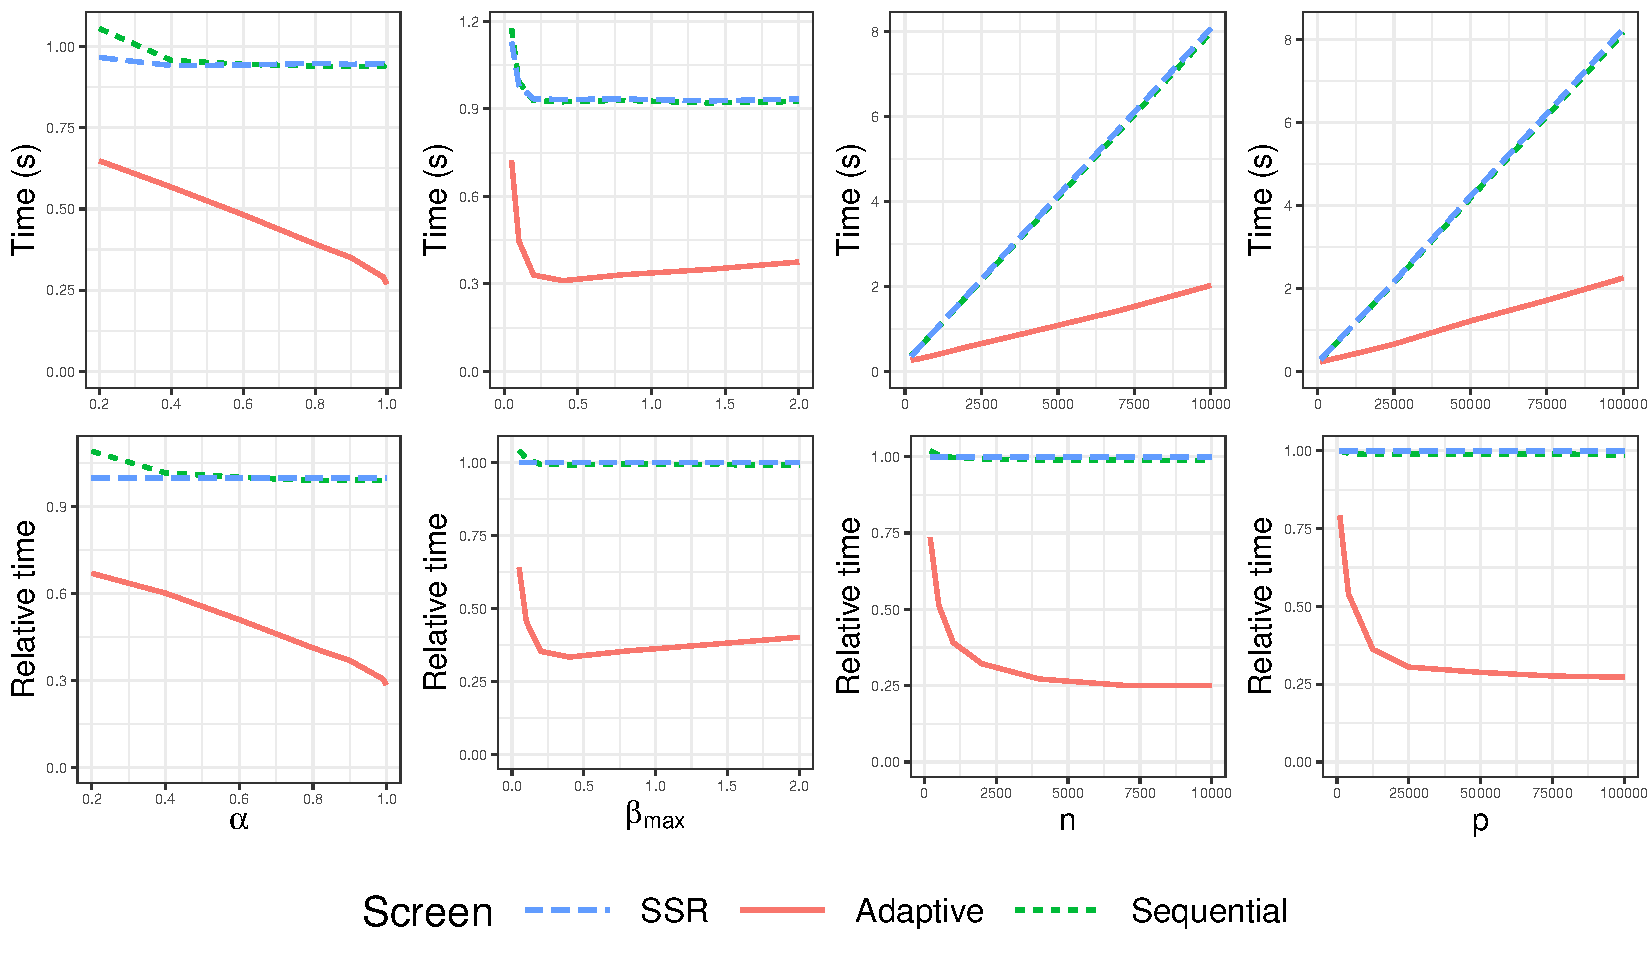
\includegraphics[width=\textwidth]{enet1.pdf}    \caption{Comparing speed of screening methods for elastic model under different settings. Top row: computation time in second. Bottom row: relative computation time compared to SSR. First column: Varying proportion of lasso penalty: $\alpha$. Second column: varying sample size $n$. Third column: varying number of features $p$. Fourth column: varying signal strength $\beta_{\max}$.}
    \label{fig:sim1}
\end{figure}

\begin{figure}[ht]
    \centering
    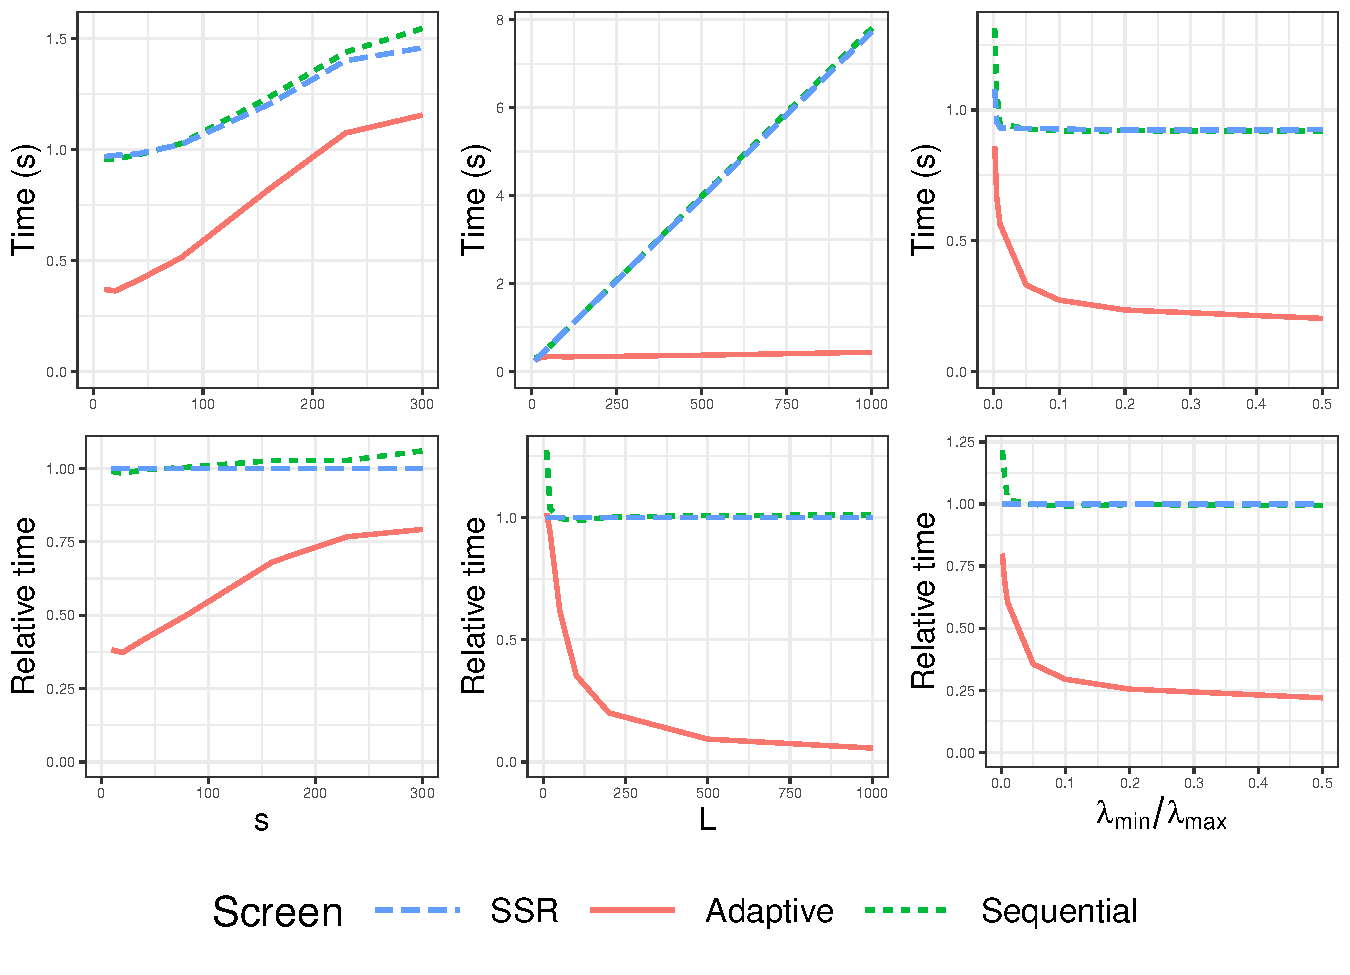
\includegraphics[width=0.82\textwidth]{enet2.pdf}    \caption{Comparing speed of screening methods for elastic net model under different settings. Top row: computation time in second. Bottom row: relative computation time compared to SSR. First column: varying sparsity $s$. Second column: Varying number of grid points $L$. Third column: Varying range of grid $\lambda_{\min}/\lambda_{\max}$.}
    \label{fig:sim2}
\end{figure}

The time spent on solving the whole path in seconds and the relative time compared to SSR method is summarized in Figure \ref{fig:sim1} and \ref{fig:sim2}. First, the sequential version of our proposed screening rule performs almost the same as SSR except in some extreme cases, and the adaptive version of our proposed screening rule outperforms the other two methods universally, with 3-4 $\times$ speedup in most cases. Second, the proposed adaptive method has the best performance when $\alpha$ is close to $1$. An $\alpha$ close to $1$ is a typical choice in practice because elastic problem becomes close to lasso problem and produces more sparse solution. Also, note $\alpha=1$, which corresponds to the lasso problem, is also included in the experiment, showing that our proposed method smoothly extends from lasso problem to a larger class of elastic net problem. Third, other factors show the adaptive screening is most favorable in a high-dimensional setting with large data size $n,p$ and small number of truly active features $s$ and in a path where $\lambda$ values are closely spaced when either the number of points on path $L$ is large or the path focuses on larger $\lambda$ values (larger $\lambda_{\min}/\lambda_{\max}$). Last, the effect of the signal strength $\boldsymbol\beta_{\max}$ has an interesting pattern. One would expect as the signal strengthens, screening methods should perform better at detecting 0 coefficients, which is true in the first halve of the range of $\boldsymbol\beta_{\max}$. After that, however, $\boldsymbol\beta_{\max}$ seems to have a negative effect on the adaptive method. The reason may be that we introduce an extra variable $\boldsymbol\gamma$ and result in a screening rule that is loose when $\boldsymbol\beta$ is large. Nevertheless, the adaptive method is still much faster than other methods regardless of the signal strength. We have also checked other factors, such as auto-correlation or block-correlation structure of the feature $X$ and number of threads in parallel computing, but we won't show the results here as there is no interesting pattern.

\subsection{Real Data}

\subsubsection{Traditional Data Sets}

In the section we compare the 3 screening methods on 4 real data sets that have traditional high-dimensional structures. An elastic net problem is solved along a grid of $L=100$ $\lambda$ values equally spaced on log scale between $(\lambda_{\max},\lambda_{\min}]$ where $\lambda_{\max}$ is determined by data and $\lambda_{\min}/\lambda_{\max}=0.05$. The 4 data sets are:

\begin{enumerate}
    \item \textbf{Breast cancer gene expression data
(GENE, \url{https://myweb.uiowa.edu/pbreheny/data/bcTCGA.html}):} this data has expression measurements of $p=17,322$ genes from $n=536$ patients. The response is the expression measurement of the gene BRCA1, which has been identified to be related to risk of breast cancer.
    \item \textbf{Cardiac fibrosis genome-wide association data
(GWAS, \url{https://arxiv.org/abs/1607.05636}):} this data set has $p=660,496$ single nucleotide
polymorphisms (SNPs) collected from $n=313$ human hearts. The response is the log of the ratio of cardiomyocytes to fibroblasts in the heart tissue, which is associated with heart failure.
    \item \textbf{MNIST handwritten image data
(MNIST, \url{http://yann.lecun.com/exdb/mnist}):} this data set has $60,000$ images in the training set and $10,000$ images in the testing set. Each image is a $28\times 28=784$ pixels image of handwritten digits. We use the training set to form a $n=784\times p=60,000$ feature matrix, treating pixels as samples and images as features. Then an image from the testing set is randomly selected as the response.
    \item \textbf{Subset of New York Times bag-of-words data
(NYT, \url{https://archive.ics.uci.edu/ml/datasets/Bag+of+Words}):} the raw data set is a $300,000\times 102,660$ matrix, each row being a document and each column being number of occurrence of a specific word in those documents. We selected $n=5,500$ documents by removing documents with low word counts. Then $55,000$ words are selected as the features and a randomly selected word is the response.
\end{enumerate}

For the GENE and GWAS data sets, the experiment is replicated 10 times, and the for the MNIST and NYT data sets, because the response is randomly selected, the experiment is replicated 50 times. The Figure \ref{fig:real} summarizes the comparison of time spent on solving the whole path with different screening methods and $\alpha$ values on the 4 data sets. The proposed adaptive method is the fastest especially when $\alpha$ is close to 1. Even if $\alpha$ is small, the adaptive is still the fastest most of the times.

\begin{figure}[ht]
    \centering
    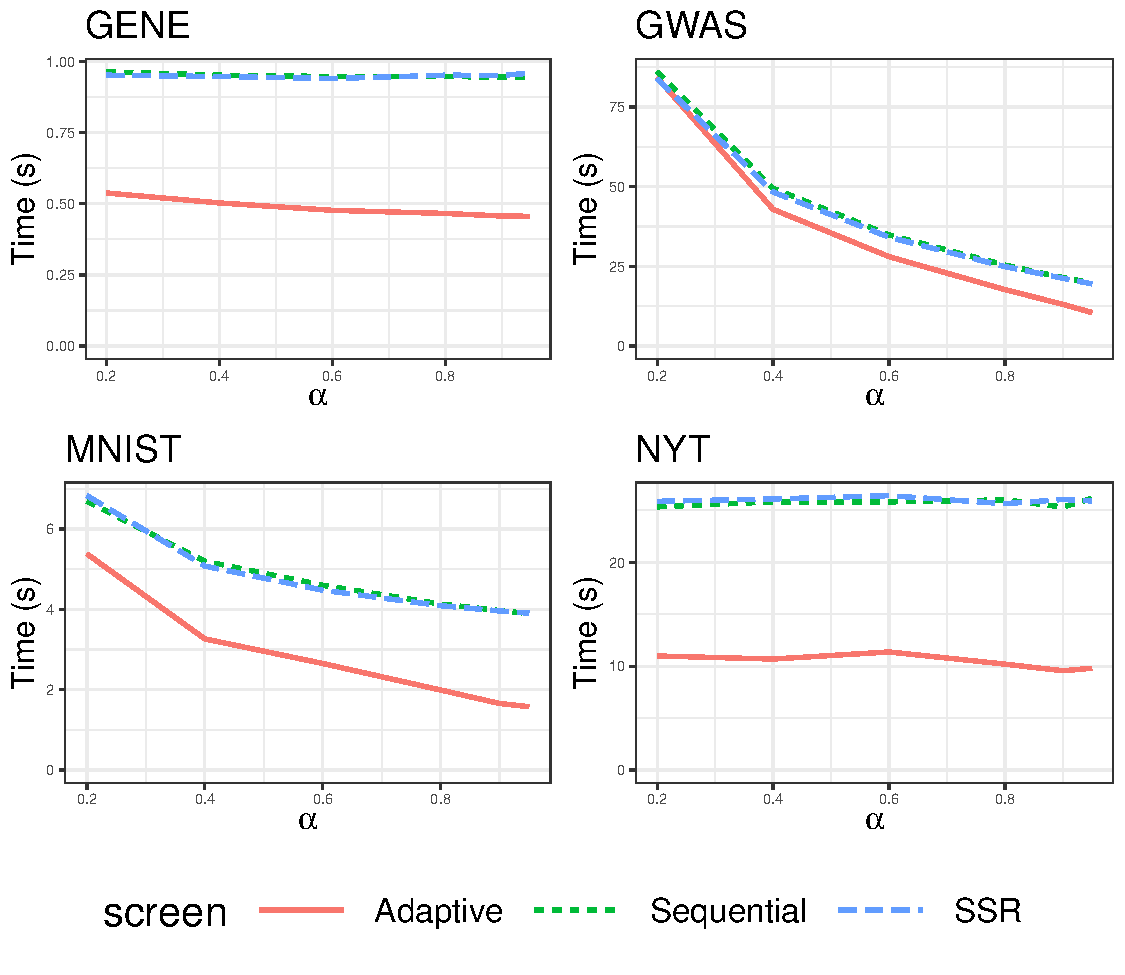
\includegraphics[width=0.82\textwidth]{enetreal.pdf}    \caption{Average computing time in seconds with different screening methods and $\alpha$ for elastic net model on 4 data sets.}
    \label{fig:real}
\end{figure}

\iffalse
\begin{table}[ht]
\centering
\begin{tabular}{llll}
\toprule
Screening method & SSR & Sequential & Adaptive  \\
\midrule
$\alpha=0.95$ & 945 (4) & 949 (3) & \textbf{455 (2)} \\
$\alpha=0.9$ & 946 (3) & 949 (4) & \textbf{465 (2)}  \\
$\alpha=0.8$ & 939 (2) & 948 (2) & \textbf{471 (2)}  \\
$\alpha=0.6$ & 936 (2) & 949 (2) & \textbf{485 (2)}  \\
$\alpha=0.4$ & 938 (1) & 949 (1) & \textbf{500 (1)}  \\
$\alpha=0.2$ & 953 (4) & 966 (2) & \textbf{544 (3)} \\
\bottomrule
\end{tabular}
\caption{Average computing time in millisecond (standard error) for the GENE data set}
\label{Tab:gene}
\end{table}
\fi

\subsubsection{Ultra High-dimensional Data Sets}

In this section, we consider a ultra high-dimensional real data set that cannot be fit into the memory. This scenario is the greatest challenge to an optimizing algorithm and a good screening method will be most wanted. The data from the Genetic Risk Assessment of Defibrillator Events study (GRADE, \url{https://www.clinicaltrials.gov/ct2/show/NCT02045043}) is a genome-wide genetic data and were collected for 1,080 subjects diagnosed with cardiomyopathy and who had undergone surgery to receive an implantable cardioverter defibrillator in the past 5 years. After imputation using the Haplotype Reference Consortium as a reference genome and filtering for quality control \citep{Das2016}, there were $p=11,830,470$ SNPs which used as features. The size of the file storing the feature matrix is 96G and we conduct the test on a machine with 32G RAM. A variety of clinical data was collected on these individuals. To examine the performance of screening methods for elastic net problem, we focused on the numeric response left ventricular ejection fraction (LVEF). LVEF measures the proportion of blood being pumped out of the left ventricle of the heart with each contraction. Lower values are associated with more severe heart disease. LVEF data was available for $n=973$ subjects and they will be considered as the sample for this analysis. We chose a relatively large $\lambda_{\min} =0.1\lambda_{\max}$ to avoid having much more features selected than the number of observations. This choice will lead to a solution path with $1106$ to $4791$ features selected at the end of the path, depending on the value of $\alpha$. We choose number of $\lambda$ values to be the default value $L=100$ and test a grid of $\alpha$ values $\{1,0.95,0.9,0.8,0.6,0.4,0.2\}$. The time spent to solve the whole path in minutes for different screening methods and $\alpha$'s is shown in Figure~\ref{fig:lvef}. 

\begin{figure}[ht]
    \centering
    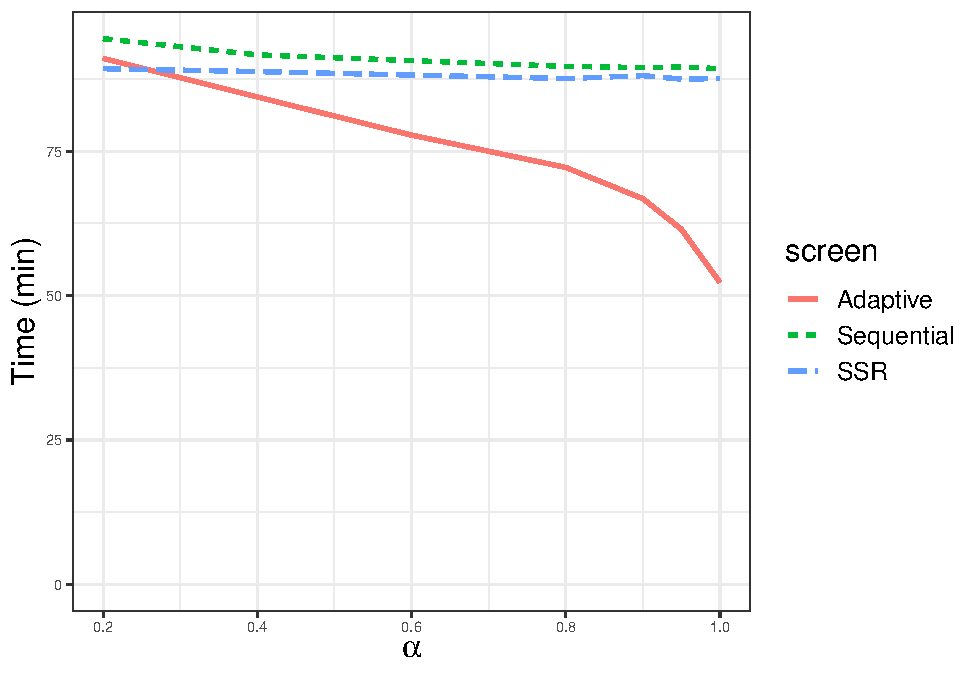
\includegraphics[width=0.72\textwidth]{enetlvef.pdf}    \caption{Average computing time in minutes with different screening methods and $\alpha$ for elastic net model on GRADE data set.}
    \label{fig:lvef}
\end{figure}

\iffalse
\begin{table}[ht]
\centering
\begin{tabular}{llllll}
\toprule
Screening method & SSR\,\,\,\,\,\,\,\,\,    & Sequential   & Adaptive  \\
\midrule
$\alpha=1$ & 87.6 & 89.3 & \textbf{52.3}  \\
$\alpha=0.95$ & 87.5 & 89.6 & \textbf{61.5}  \\
$\alpha=0.9$ & 88.1 & 89.5 & \textbf{66.8}  \\
$\alpha=0.8$ & 87.6 & 89.7 & \textbf{72.2}  \\
$\alpha=0.6$ & 88.2 & 90.7 & \textbf{77.8} \\
$\alpha=0.4$ & 88.8 & 91.7 & \textbf{84.4}  \\
$\alpha=0.2$ & \textbf{89.3} & 94.5 & 91.1  \\

\bottomrule
\end{tabular}
\caption{Average computing time in minutes the LVEF analysis with elastic net.\label{Tab:lvef}}
\end{table}
\fi

The proposed adaptive screening is the fastest in most cases, especially in the case when $\alpha$ is large. Even if $\alpha$ is extremely small, it does not do much harm to the speed. The proposed sequential screening performs very similar to strong rule screening.

\section{Discussion}

In this paper, we derive a safe screening rule for pathwise elastic net problem that utilizes previous solution as a reference for enhanced screening power by considering an intermediate problem that connects the reference and the target. We show that it can be built into a adaptive screening method that performs 3-4 times faster than the other state-of-the-art method SSR in most cases. The adaptive method is implemented in the public available \textbf{biglasso} R package.

Our result covers the more popular used form of elastic net problem \eqref{eq:enet}. This form is not only more useful in practice, but is also mathematical more interesting because it cannot be reduced to lasso problem. In fact our proposed safe screening method is the only existing method we know of that works on penalty function with varying shape as $\lambda$ varies. A constant shape penalty $\lambda p(\boldsymbol\beta)$, such as lasso penalty or group lasso penalty can be rewritten as $p(\lambda\boldsymbol\beta)$, but the elastic net penalty does not share this property. Our result suggests possibility on a larger family of penalty functions.

Besides the standard elastic net problem we have covered, there is also a family of elastic net penalized generalized linear regression problems that can benefit from screening, but as far as we know, the strong rule screening is the only available screening method for these problems. Since our derivation has already tackled the trickiest part which is the varying shape of elastic net penalty function, similar technique can also help to derive safe rule and thus adaptive safe screening for elastic net penalized generalized regression problems, such as elastic net penalized logistic regression.

\appendix
\appendixpage

\section{Derivation of the Dual Problem}
\label{sec:dual}

Introducing 2 new variables $\boldsymbol r\equiv \boldsymbol y-X\boldsymbol\beta$ and $\boldsymbol b\equiv n(1-\alpha)\lambda \boldsymbol\beta$, then the problem \eqref{eq:enet} becomes:

\begin{equation}
    \label{eq:dual+rb}
    \begin{gathered}
    \underset{\boldsymbol\beta\in \mathbb{R}^p}{\mathrm{min}}\frac{1}{2}||\boldsymbol r||_2^2+\frac{1}{2n(1-\alpha)\lambda}||\boldsymbol b||_2^2+n\alpha\lambda||\boldsymbol\beta||_1\\s.t.\quad \boldsymbol r=\boldsymbol y-X\boldsymbol\beta,\quad \boldsymbol b=n(1-\alpha)\lambda \boldsymbol\beta.
\end{gathered}
\end{equation}
Introducing the dual variables $\boldsymbol u\in\mathbb{R}^{n},\boldsymbol w\in\mathbb{R}^p$, the dual problem becomes:

\begin{gather}
    \label{eq:dual+uw}
    \begin{aligned}
        &\underset{\boldsymbol u,\boldsymbol w}{\mathrm{max}}\,\underset{\boldsymbol r,\boldsymbol b}{\mathrm{min}}\,\underset{\boldsymbol\beta}{\mathrm{min}}\,\frac{1}{2}||\boldsymbol r||_2^2+\frac{1}{2n(1-\alpha)\lambda}||\boldsymbol b||_2^2+n\alpha\lambda||\boldsymbol\beta||_1+\boldsymbol u^T(\boldsymbol y-X\boldsymbol\beta-\boldsymbol r)+\boldsymbol w^T\left(\boldsymbol\beta-\frac{\boldsymbol b}{n(1-\alpha)\lambda}\right)\\
        =&\underset{\boldsymbol u,\boldsymbol w}{\mathrm{max}}\,\underset{\boldsymbol r,\boldsymbol b}{\mathrm{min}}\,\underset{\boldsymbol\beta}{\mathrm{min}}\,n\alpha\lambda||\boldsymbol\beta||_1-\boldsymbol u^TX\boldsymbol\beta+\boldsymbol w^T\boldsymbol\beta+\frac{1}{2}||\boldsymbol r||_2^2+\boldsymbol u^T(\boldsymbol y-\boldsymbol r)+\frac{1}{2n(1-\alpha)\lambda}||\boldsymbol b||_2^2-\frac{\boldsymbol w^T\boldsymbol b}{n(1-\alpha)\lambda}
    \end{aligned}    
\end{gather}
Minimizing with respect to $\boldsymbol\beta$, the partial derivative is:

\begin{equation}
    \label{eq:partialbeta}
    \frac{\partial}{\partial\boldsymbol\beta}(\cdot) =-X^T\boldsymbol u+\boldsymbol w+n\alpha\lambda\frac{\partial||\boldsymbol\beta||_1}{\partial\boldsymbol\beta},
\end{equation}
so the minimum is obtained iff $||X^T\boldsymbol u-\boldsymbol w||_\infty\leq n\alpha\lambda,$ and the problem becomes:

\begin{gather}
    \label{eq:dualuw}
    \begin{aligned}
        &\underset{\boldsymbol u,\boldsymbol w}{\mathrm{max}}\,\underset{\boldsymbol r,\boldsymbol b}{\mathrm{min}}\,\frac{1}{2}||\boldsymbol r||_2^2+\boldsymbol u^T(\boldsymbol y-\boldsymbol r)+\frac{1}{2n(1-\alpha)\lambda}||\boldsymbol b||_2^2-\frac{\boldsymbol w^T\boldsymbol b}{n(1-\alpha)\lambda}\\
        =&\underset{\boldsymbol u,\boldsymbol w}{\mathrm{max}}\,\underset{\boldsymbol r,\boldsymbol b}{\mathrm{min}}\,\frac{1}{2}||\boldsymbol r-\boldsymbol u||_2^2+\boldsymbol u^T\boldsymbol y-\frac{1}{2}||\boldsymbol u||_2^2+\frac{1}{2n(1-\alpha)\lambda}||\boldsymbol b-\boldsymbol w||_2^2-\frac{1}{2n(1-\alpha)\lambda}||\boldsymbol w||_2^2\\
        =&\underset{\boldsymbol u,\boldsymbol w}{\mathrm{max}}\,\underset{\boldsymbol r,\boldsymbol b}{\mathrm{min}}\,\frac{1}{2}||\boldsymbol r-\boldsymbol u||_2^2+\frac{1}{2}||\boldsymbol y||_2^2-\frac{1}{2}||\boldsymbol u-\boldsymbol y||_2^2+\frac{1}{2n(1-\alpha)\lambda}||\boldsymbol b-\boldsymbol w||_2^2-\frac{1}{2n(1-\alpha)\lambda}||\boldsymbol w||_2^2\\
        =&\underset{\boldsymbol u,\boldsymbol w}{\mathrm{max}}\,\frac{1}{2}||\boldsymbol y||_2^2-\frac{1}{2}||\boldsymbol u-\boldsymbol y||_2^2-\frac{1}{2n(1-\alpha)\lambda}||\boldsymbol w||_2^2,
    \end{aligned}
\end{gather}
where the minimum is obtained iff $\boldsymbol r=\boldsymbol u$ and $\boldsymbol b=\boldsymbol w$. Letting $\boldsymbol\theta\equiv\frac{\boldsymbol u}{\lambda}=\frac{\boldsymbol y-X\boldsymbol\beta}{\lambda}$ and $\boldsymbol\gamma\equiv\frac{\boldsymbol w}{\sqrt{n(1-\alpha)\lambda^3}}=\sqrt{\frac{n(1-\alpha)}{\lambda}}\boldsymbol\beta$, the problem becomes the dual problem in \eqref{eq:dualtheta} and the dual solution and primal solution can be connected by \eqref{eq:dualprimal}.

\section{Proof of Theorem \ref{thm:1.1}}


Considering the second order expansion of $g_{\lambda_0}$ at $(\boldsymbol\theta_{0},\boldsymbol\gamma_{0})$, $g_{\lambda_0}\left(\boldsymbol\theta_{1|0},\sqrt{\frac{\lambda_1}{\lambda_0}}\boldsymbol\gamma_{1|0}\right)$ can be written as

\begin{equation}
    \label{eq:1.1.1}
    g_{\lambda_0}\binom{\boldsymbol\theta_{1|0}}{\sqrt{\frac{\lambda_1}{\lambda_0}}\boldsymbol\gamma_{1|0}}=g_{\lambda_0}\binom{\boldsymbol\theta_{0}}{\boldsymbol\gamma_{0}}+\left\langle\nabla g_{\lambda_0}\binom{\boldsymbol\theta_{0}}{\boldsymbol\gamma_{0}},\binom{\boldsymbol\theta_{1|0}}{\sqrt{\frac{\lambda_1}{\lambda_0}}\boldsymbol\gamma_{1|0}}-\binom{\boldsymbol\theta_{0}}{\boldsymbol\gamma_{0}}\right\rangle-\frac{\lambda_0^2}{2}\left\Vert\binom{\boldsymbol\theta_{1|0}}{\sqrt{\frac{\lambda_1}{\lambda_0}}\boldsymbol\gamma_{1|0}}-\binom{\boldsymbol\theta_{0}}{\boldsymbol\gamma_{0}}\right\Vert_2^2,
\end{equation}
because $\nabla^2g_{\lambda_0}$ is $-\lambda_0^2$ times the identity matrix. 

First, both $(\boldsymbol\theta_{0},\boldsymbol\gamma_{0})$ and $\left(\boldsymbol\theta_{1|0},\sqrt{\frac{\lambda_1}{\lambda_0}}\boldsymbol\gamma_{1|0}\right)$ are in the convex set $\mathcal{F}_{\lambda_0}$. The latter is true because

\begin{equation}
    \left\Vert X^T\boldsymbol\theta_{\lambda_1|\lambda_0}-\sqrt{n(1-\alpha)\lambda_0}\sqrt{\frac{\lambda_1}{\lambda_0}}\boldsymbol\gamma_{\lambda_1|\lambda_0}\right\Vert_\infty= \left\Vert X^T\boldsymbol\theta_{\lambda_1|\lambda_0}-\sqrt{n(1-\alpha)\lambda_1}\boldsymbol\gamma_{\lambda_1|\lambda_0}\right\Vert_\infty\leq n\alpha.
\end{equation}
$(\boldsymbol\theta_{0},\boldsymbol\gamma_{0})$ is the maximizer in the convex set $\mathcal{F}_{\lambda_0}$ so it must satisfy the first order condition:

\begin{equation}
    \label{eq:1.1.2}
    \left\langle\nabla g_{\lambda_0}\binom{\boldsymbol\theta_{0}}{\boldsymbol\gamma_{0}},\binom{\boldsymbol\theta_{1|0}}{\sqrt{\frac{\lambda_1}{\lambda_0}}\boldsymbol\gamma_{1|0}}-\binom{\boldsymbol\theta_{0}}{\boldsymbol\gamma_{0}}\right\rangle\leq 0,
\end{equation}
because if not, $(\boldsymbol\theta_{0},\boldsymbol\gamma_{0})$ can be improved by moving by a small amount towards the direction of\newline $\left(\boldsymbol\theta_{1|0},\sqrt{\frac{\lambda_1}{\lambda_0}}\boldsymbol\gamma_{1|0}\right)-(\boldsymbol\theta_{0},\boldsymbol\gamma_{0})$. Combining it with \eqref{eq:1.1.1}:

\begin{equation}
    \label{eq:1.1.3}
    g_{\lambda_0}\binom{\boldsymbol\theta_{0}}{\boldsymbol\gamma_{0}}\geq g_{\lambda_0}\binom{\boldsymbol\theta_{1|0}}{\sqrt{\frac{\lambda_1}{\lambda_0}}\boldsymbol\gamma_{1|0}}+\frac{\lambda_0^2}{2}\left\Vert\binom{\boldsymbol\theta_{1|0}}{\sqrt{\frac{\lambda_1}{\lambda_0}}\boldsymbol\gamma_{1|0}}-\binom{\boldsymbol\theta_{0}}{\boldsymbol\gamma_{0}}\right\Vert_2^2.
\end{equation}

Second, by the same argument, both $(\boldsymbol\theta_{1|0},\boldsymbol\gamma_{1|0})$ and $\left(\boldsymbol\theta_{0},\sqrt{\frac{\lambda_0}{\lambda_1}}\boldsymbol\gamma_{0}\right)$ are in the convex set $\mathcal{F}_{\lambda_1}$, and we have the same result as \eqref{eq:1.1.3}:

\begin{equation}
    \label{eq:1.1.4}
    g_{\lambda_0}\binom{\boldsymbol\theta_{1|0}}{\boldsymbol\gamma_{1|0}}\geq g_{\lambda_0}\binom{\boldsymbol\theta_{0}}{\sqrt{\frac{\lambda_0}{\lambda_1}}\boldsymbol\gamma_{0}}+\frac{\lambda_0^2}{2}\left\Vert\binom{\boldsymbol\theta_{0}}{\sqrt{\frac{\lambda_0}{\lambda_1}}\boldsymbol\gamma_{0}}-\binom{\boldsymbol\theta_{1|0}}{\boldsymbol\gamma_{1|0}}\right\Vert_2^2.
\end{equation}

Then,

\begin{gather}
    \label{eq:1.1.5}
    \begin{aligned}
        g_{\lambda_0}\binom{\boldsymbol\theta_{1|0}}{\sqrt{\frac{\lambda_1}{\lambda_0}}\boldsymbol\gamma_{1|0}}&=\frac{1}{2}||\boldsymbol y||_2^2-\frac{\lambda_0^2}{2}\left\Vert\frac{\boldsymbol y}{\lambda_0}-\boldsymbol\theta_{1|0}\right\Vert_2^2-\frac{\lambda_1\lambda_0}{2}||\boldsymbol\gamma_{1|0}||_2^2\\
        &= \frac{1}{2}||\boldsymbol y||_2^2-\frac{\lambda_0^2}{2}\left\Vert\frac{\boldsymbol y}{\lambda_0}-\boldsymbol\theta_{1|0}\right\Vert_2^2-\frac{\lambda_0^2}{2}||\boldsymbol\gamma_{1|0}||_2^2+\left(\frac{\lambda_0^2}{2}-\frac{\lambda_1\lambda_0}{2}\right)||\boldsymbol\gamma_{1|0}||_2^2\\
        &=g_{\lambda_0}\binom{\boldsymbol\theta_{1|0}}{\boldsymbol\gamma_{1|0}}+\frac{\lambda_0(\lambda_0-\lambda_1)}{2}||\boldsymbol\gamma_{1|0}||_2^2\\
        &\geq g_{\lambda_0}\binom{\boldsymbol\theta_{0}}{\sqrt{\frac{\lambda_0}{\lambda_1}}\boldsymbol\gamma_{0}}+\frac{\lambda_0(\lambda_0-\lambda_1)}{2}||\boldsymbol\gamma_{1|0}||_2^2+\frac{\lambda_0^2}{2}\left\Vert\binom{\boldsymbol\theta_{0}}{\sqrt{\frac{\lambda_0}{\lambda_1}}\boldsymbol\gamma_{0}}-\binom{\boldsymbol\theta_{1|0}}{\boldsymbol\gamma_{1|0}}\right\Vert_2^2\\
        &=g_{\lambda_0}\binom{\boldsymbol\theta_{0}}{\boldsymbol\gamma_{0}}-\frac{\lambda_0^2(\lambda_0-\lambda_1)}{2\lambda_1}||\boldsymbol\gamma_{0}||_2^2+\frac{\lambda_0(\lambda_0-\lambda_1)}{2}||\boldsymbol\gamma_{1|0}||_2^2+\frac{\lambda_0^2}{2}\left\Vert\binom{\boldsymbol\theta_{0}}{\sqrt{\frac{\lambda_0}{\lambda_1}}\boldsymbol\gamma_{0}}-\binom{\boldsymbol\theta_{1|0}}{\boldsymbol\gamma_{1|0}}\right\Vert_2^2,
    \end{aligned}
\end{gather}
where the inequality is due to \eqref{eq:1.1.4}. Combining \eqref{eq:1.1.3} and \eqref{eq:1.1.5} we have:

\begin{gather}
    \begin{aligned}
        &\left\Vert\binom{\boldsymbol\theta_{0}}{\sqrt{\frac{\lambda_0}{\lambda_1}}\boldsymbol\gamma_{0}}-\binom{\boldsymbol\theta_{1|0}}{\boldsymbol\gamma_{1|0}}\right\Vert_2^2+\left\Vert\binom{\boldsymbol\theta_{1|0}}{\sqrt{\frac{\lambda_1}{\lambda_0}}\boldsymbol\gamma_{1|0}}-\binom{\boldsymbol\theta_{0}}{\boldsymbol\gamma_{0}}\right\Vert_2^2\leq c\lambda_0||\boldsymbol\gamma_{_0}||_2^2-c\lambda_1||\boldsymbol\gamma_{1|0}||_2^2,
    \end{aligned}
\end{gather}
and rearranging the terms

\begin{gather}
    \begin{aligned}
        &2||\boldsymbol\theta_{1|0}-\boldsymbol\theta_{0}||_2^2\\\leq& c\lambda_0||\boldsymbol\gamma_{0}||_2^2-c\lambda_1||\boldsymbol\gamma_{1|0}||_2^2-\left\Vert\sqrt{\frac{\lambda_1}{\lambda_0}}\boldsymbol\gamma_{1|0}-\boldsymbol\gamma_{0}\right\Vert_2^2-\left\Vert\sqrt{\frac{\lambda_0}{\lambda_1}}\boldsymbol\gamma_{0}-\boldsymbol\gamma_{1|0}\right\Vert_2^2\\
        =&c\lambda_0||\boldsymbol\gamma_{0}||_2^2-c\lambda_1||\boldsymbol\gamma_{1|0}||_2^2-\left(1+\frac{\lambda_1}{\lambda_0}\right)||\boldsymbol\gamma_{1|0}||_2^2+2\left(\sqrt{\frac{\lambda_1}{\lambda_0}}+\sqrt{\frac{\lambda_0}{\lambda_1}}\right)\boldsymbol\gamma_{0}^T\boldsymbol\gamma_{1|0}-\left(1+\frac{\lambda_0}{\lambda_1}\right)||\boldsymbol\gamma_{0}||_2^2\\
        =&-2||\boldsymbol\gamma_{1|0}||_2^2+4d\boldsymbol\gamma_{0}^T\gamma_{1|0}-2||\boldsymbol\gamma_{0}||_2^2\\
        =&-2\left\Vert\boldsymbol\gamma_{1|0}-d\boldsymbol\gamma_{0}\right\Vert_2^2+2(d^2-1)||\boldsymbol\gamma_{0}||_2^2\\
    \end{aligned}
\end{gather}
where $d\equiv \frac{\sqrt{\frac{\lambda_1}{\lambda_0}}+\sqrt{\frac{\lambda_0}{\lambda_1}}}{2}$. It leads to the same result as in the theorem

\begin{equation}
     \left\Vert\binom{\boldsymbol\theta_{1|0}}{\boldsymbol\gamma_{1|0}}-\binom{\boldsymbol\theta_{0}}{d\boldsymbol\gamma_{0}}\right\Vert_2^2\leq (d^2-1)||\boldsymbol\gamma_{0}||_2^2.
\end{equation}

\section{Proof of Theorem \ref{thm:1.2}}

From a geometric aspect, the dual problem \eqref{eq:dualtheta} is minimizing an $L_2$ distance, or in other word, finding a projection. $\boldsymbol\mu_{1|0}=(\boldsymbol \theta_{1|0},\boldsymbol \gamma_{1|0})$ is the projection of $(\frac{\boldsymbol y}{\lambda_0},\boldsymbol0)$ onto $\mathcal{F}_{\lambda_1}$ while $\boldsymbol\mu_1=(\boldsymbol \theta_{1},\boldsymbol \gamma_{1})$ is the projection of $(\frac{\boldsymbol y}{\lambda_1},\boldsymbol0)$ onto the same set $\mathcal{F}_{\lambda_1}$. $\mathcal{F}_{\lambda_1}$ is a nonempty closed convex set. We define

\begin{gather}
    \label{eq:1.2.1}
    \begin{aligned}
        \boldsymbol v_1\equiv\binom{\frac{\boldsymbol y}{\lambda_0}-\boldsymbol \theta_{1|0}}{-\boldsymbol \gamma_{1|0}}=\binom{\frac{\boldsymbol y}{\lambda_0}}{\boldsymbol0}-\boldsymbol\mu_{1|0},\\
        \boldsymbol v_2\equiv \binom{\frac{\boldsymbol y}{\lambda_1}-\boldsymbol \theta_{1|0}}{-\boldsymbol \gamma_{1|0}}=\binom{\frac{\boldsymbol y}{\lambda_1}}{\boldsymbol0}-\boldsymbol\mu_{1|0}.
    \end{aligned}
\end{gather}

First, we have the idea of projections of rays, stated as the following

\begin{lemma}
    \citep{Bauschke2011}
    Let $\mathcal{C}$ be a nonempty closed convex subset of a Hilbert space $\mathcal{H}$. For any $\boldsymbol w\in\mathcal{H}$ , let $P_{\mathcal{C}}(\boldsymbol w)$ be the projection of $\boldsymbol w$ onto $\mathcal{C}$. Then for any $\boldsymbol w\in\mathcal{H}$ and $t\geq 0$,
    \begin{equation}
        P_{\mathcal{C}}\left(P_{\mathcal{C}}(\boldsymbol w)+t\left(\boldsymbol w-P_{\mathcal{C}}(\boldsymbol w)\right)\right)=P_{\mathcal{C}}(\boldsymbol w).
    \end{equation}
\end{lemma}

If we choose $\boldsymbol w=(\frac{\boldsymbol y}{\lambda_0},\boldsymbol0)$, it says for all $t\geq 0$, $\boldsymbol\mu_{1|0}$ is also the projection of $\boldsymbol\mu_{1|0}+t\boldsymbol v_1$ onto $\mathcal{F}_{\lambda_1}$. Next we also have the firmly nonexpansiveness property of projections:

\begin{lemma}
    \citep{Bauschke2011}
    Let $\mathcal{C}$ be a nonempty closed convex subset of a Hilbert space $\mathcal{H}$. For any $\boldsymbol w_1,\boldsymbol w_2\in\mathcal{H}$,
    \begin{equation}
        ||P_{\mathcal{C}}(\boldsymbol w_1)-P_{\mathcal{C}}(\boldsymbol w_2)||_2^2\leq \langle\boldsymbol w_1-\boldsymbol w_2, P_{\mathcal{C}}(\boldsymbol w_1)-P_{\mathcal{C}}(\boldsymbol w_2)\rangle.
    \end{equation}
\end{lemma}

If we rearrange the terms into squares, it says:

\begin{equation}
    ||P_{\mathcal{C}}(\boldsymbol w_1)-P_{\mathcal{C}}(\boldsymbol w_2)-\frac{1}{2}(\boldsymbol w_1-\boldsymbol w_2)||_2^2\leq\frac{1}{4}||\boldsymbol w_1-\boldsymbol w_2||_2^2.
\end{equation}

If we choose $\boldsymbol w_1=(\frac{\boldsymbol y}{\lambda_1},\boldsymbol0),\boldsymbol w_2=\boldsymbol\mu_{1|0}+t\boldsymbol v_1$, which means $P_{\mathcal{C}}(\boldsymbol w_1)=\boldsymbol\mu_1,P_{\mathcal{C}}(\boldsymbol w_2)=\boldsymbol\mu_{1|0},\boldsymbol w_1-\boldsymbol w_2=\boldsymbol v_2-t\boldsymbol v_1$, we have:

\begin{equation}
    \left\Vert\boldsymbol\mu_1-\boldsymbol\mu_{1|0}-\frac{1}{2}(\boldsymbol v_2-t\boldsymbol v_1)\right\Vert_2^2\leq\frac{1}{4}||\boldsymbol v_2-t\boldsymbol v_1||_2^2,
\end{equation}
which means $\boldsymbol\mu_1=(\boldsymbol\theta_{\lambda_1},\boldsymbol\gamma_{\lambda_1})$ is bounded in a ball. Plugging in the definition in \eqref{eq:1.2.1} will result in the form stated in the theorem.

\section{Proof of Theorem \ref{thm:2.1}}

The maximum of $\Tilde{T}^\xi_j$ can be bounded by the sum of two maximums:

\begin{equation}
    \begin{gathered}
        \underset{\boldsymbol\mu'\in\mathcal{A}^1}{\mathrm{max}}\Tilde{T}^\xi_j(\lambda_1,\lambda_0,t|\boldsymbol\mu')\\
        =\underset{\boldsymbol\mu'\in\mathcal{A}^1}{\mathrm{max}}\left[\xi\left( \frac{1}{2}(\frac{1-t}{\lambda_0}+c)\boldsymbol x_j^T\boldsymbol y+\frac{t+1}{2}\boldsymbol x_j^T\boldsymbol\theta'\right)+\frac{||\boldsymbol x_j||_2|1-t|}{2}\left\Vert\binom{\boldsymbol\theta'-\left(\frac{1}{\lambda_0}+\frac{c}{1-t}\right)\boldsymbol y}{\boldsymbol\gamma'}\right\Vert_2\right]\\
        \leq \underset{\boldsymbol\mu'\in\mathcal{A}^1}{\mathrm{max}}\xi\left( \frac{1}{2}(\frac{1-t}{\lambda_0}+c)\boldsymbol x_j^T\boldsymbol y+\frac{t+1}{2}\boldsymbol x_j^T\boldsymbol\theta'\right)+\underset{\boldsymbol\mu'\in\mathcal{A}^1}{\mathrm{max}}\frac{||\boldsymbol x_j||_2|1-t|}{2}\left\Vert\binom{\boldsymbol\theta'-\left(\frac{1}{\lambda_0}+\frac{c}{1-t}\right)\boldsymbol y}{\boldsymbol\gamma'}\right\Vert_2.
    \end{gathered}
\end{equation}

The first maximization problem is maximizing a linear function in a ball with center $\boldsymbol c_1$ and radius $r_1$, so the maximum can be easily obtained as:

\begin{gather}
    \begin{aligned}
        \frac{\frac{1-t}{\lambda_0}+c}{2}\xi\boldsymbol x_j^T \boldsymbol y+\frac{t+1}{2}\left(\xi \boldsymbol x_j^T \boldsymbol c_1^\theta+||\boldsymbol x_j||_2r_1\right)\\
        =\frac{\frac{1-t}{\lambda_0}+c}{2}\xi\boldsymbol x_j^T \boldsymbol y+\frac{t+1}{2}\left(\xi \boldsymbol x_j^T \boldsymbol \theta_{0}+||\boldsymbol x_j||_2\sqrt{d^2-1}||\boldsymbol\gamma_{0}||_2\right).
    \end{aligned}
\end{gather}

The second maximization problem is maximizing the distance to $\left((\frac{1}{\lambda_0}+\frac{c}{1-t})\boldsymbol y,\boldsymbol 0\right)$ in a ball with center $\boldsymbol c_1$ and radius $r_1$, so the maximum can also be easily obtained as:

\begin{gather}
    \begin{aligned}
        \frac{||\boldsymbol x_j||_2|1-t|}{2}\left(\left\Vert\boldsymbol c_1-\binom{(\frac{1}{\lambda_0}+\frac{c}{1-t})\boldsymbol y}{\boldsymbol 0}\right\Vert_2+r_1\right)\\
        =\frac{||\boldsymbol x_j||_2}{2}\left\Vert\binom{(1-t)\boldsymbol\theta_{0}-\left(\frac{1-t}{\lambda_0}+c\right)\boldsymbol y}{(1-t)d\boldsymbol\gamma_{0}}\right\Vert_2+\frac{||\boldsymbol x_j||_2|1-t|}{2}\sqrt{d^2-1}||\boldsymbol\gamma_0||_2.
    \end{aligned}
\end{gather}

$T^\xi_j$ is the sum of these two maximums so it is an upper bound for $\Tilde{T}^\xi_j$.

\iffalse
\section{Proof of Theorem \ref{thm:2.2}}

Defining the following quantities:
\begin{gather}
    \begin{aligned}
        \boldsymbol b_0&\equiv\binom{\frac{t+1}{2}\xi \boldsymbol x_j}{\boldsymbol 0},\\
        a_0&\equiv\frac{||\boldsymbol x_j||_2|1-t|)}{2},\\
        \boldsymbol c_0'&\equiv\binom{\left(\frac{1}{\lambda_0}+\frac{c}{1-t}\right)\boldsymbol y}{0},\\
        \boldsymbol z &\equiv \binom{\boldsymbol\theta'}{\boldsymbol\gamma'}.
    \end{aligned}
\end{gather}

Note $\boldsymbol c_1-\boldsymbol c_0'=\binom{*}{\sqrt{\frac{\lambda_1}{\lambda_0}}\boldsymbol\gamma_{\lambda_0}}$, where the last $p$ elements will be non-zero when $\beta_{\lambda_0}$ is non-zero, which will be true because $\lambda_0<\lambda_{\max}$. This shows that $\boldsymbol c_1-\boldsymbol c_0'$ and $\boldsymbol b_0$ will never be colinear.

The problem \eqref{eq:ttildexi.alt} is equivalent to maximizing
\begin{equation}
    \label{eq:2.2.1}
    \boldsymbol b_0^T\boldsymbol z+a_0||\boldsymbol z-\boldsymbol c_0'||_2
\end{equation}

subject to the ball constraint $||\boldsymbol z-\boldsymbol c_1||_2^2\leq r_1^2$.
Take derivative with respect to $\boldsymbol z$:
\begin{equation}
    \label{eq:2.2.2}
    \frac{\partial}{\partial\boldsymbol z}=\boldsymbol b_0^T+a_0\frac{\boldsymbol z-\boldsymbol c_0'}{||\boldsymbol z-\boldsymbol c_0'||_2}.
\end{equation}
\begin{enumerate}
    \item If $t>0$:
    
    The norm of the derivative \eqref{eq:2.2.2} is positive
    \begin{equation}
        \left\Vert\frac{\partial}{\partial\boldsymbol z}=\boldsymbol b_0^T+a_0\frac{\boldsymbol z-\boldsymbol c_0'}{||\boldsymbol z-\boldsymbol c_0'||_2}\right\Vert_2^2\geq ||\boldsymbol b_0||_2^2-|a_0|\left\Vert\frac{\boldsymbol z-\boldsymbol c_0'}{||\boldsymbol z-\boldsymbol c_0'||_2}\right\Vert_2^2=\frac{t+1-|1-t|}{2}||\boldsymbol x_j||_2^2>0,
    \end{equation}
    which means the maximum will not be obtained in the interior of the ball and can only be obtained on the boundary. The Lagrangian of \eqref{eq:2.2.1} is
    \begin{equation}
        L=\boldsymbol b_0^Tz+a_0||\boldsymbol z-\boldsymbol c'_0||_2-s(||\boldsymbol z-\boldsymbol c_1||_2-r_1),
    \end{equation}
    where $s\geq0$ is the Lagrangian multiplier. Take derivative with respect to $\boldsymbol z$ and set to 0:
    \begin{gather}
        \begin{aligned}
            &\frac{\partial L}{\partial \boldsymbol z}=\boldsymbol b_0+a_0\frac{\boldsymbol z-\boldsymbol c_0'}{||\boldsymbol z-\boldsymbol c_0'||_2}-s\frac{\boldsymbol z-\boldsymbol c_1}{||\boldsymbol z-\boldsymbol c_1||_2}=0\\
            \implies &\left(\frac{s}{||\boldsymbol z-\boldsymbol c_1||_2}-\frac{a_0}{||\boldsymbol z-\boldsymbol c_0'||_2}\right)(\boldsymbol z-\boldsymbol c_1)=\boldsymbol b_0+\frac{a_0(\boldsymbol c_1-\boldsymbol c_0')}{||\boldsymbol z- \boldsymbol c_0'||_2}.
        \end{aligned}
    \end{gather}
    
    Because $\boldsymbol b_0$ and $(\boldsymbol c_1-\boldsymbol c_0')$ are not colinear, the right hand side cannot be zero and thus the left hand side cannot be zero. As a result $(\boldsymbol z- \boldsymbol c_1)$ will be in the space spanned by $\boldsymbol b_0$ and $(\boldsymbol c_1-\boldsymbol c_0')$. Combine with the fact that $\boldsymbol z$ will be on the boundary of the ball, we can decompose $\boldsymbol z$ as two orthogonal parts 
    \begin{gather}
        \begin{aligned}
            &\boldsymbol z=\boldsymbol c_1+w_0 r_1\boldsymbol v_0+w_1 r_1\boldsymbol v_1,\\
            where&\quad \boldsymbol v_0\equiv\frac{\boldsymbol b_0}{||\boldsymbol b_0||_2},\, \boldsymbol v_1\equiv \frac{(\boldsymbol c_1-\boldsymbol c_0')-\frac{(\boldsymbol c_1-\boldsymbol c_0')^T\boldsymbol b_0}{||\boldsymbol b_0||_2^2}\boldsymbol b_0}{||(\boldsymbol c_1-\boldsymbol c_0')-\frac{(\boldsymbol c_1-\boldsymbol c_0')^T\boldsymbol b_0}{||\boldsymbol b_0||_2^2}\boldsymbol b_0||_2}\\
            s.t.&\quad w_0^2+w_1^2=1.
        \end{aligned}
    \end{gather}
\end{enumerate}

\section{Alternative choice of t}

\begin{theorem}
    \label{thm:2.2}
    For any $\lambda_1<\lambda_{0}\in (0,\lambda_{max})$, $j=1,2,...,p$ and $\xi=-1,1$, assuming $(\boldsymbol\theta_{\lambda_0},\boldsymbol\gamma_{\lambda_0})$ is known, if $\boldsymbol y\neq \boldsymbol 0$,
    \begin{gather}
        \begin{aligned}
            T^\xi_j(\lambda_1,\lambda_0|\boldsymbol\theta_{\lambda_0},\boldsymbol\gamma_{\lambda_0})\equiv\underset{t\geq 0}{\mathrm{min}}\,T^\xi_j(\lambda_1,\lambda_0,t|\boldsymbol\theta_{\lambda_0},\boldsymbol\gamma_{\lambda_0})=T^\xi_j(\lambda_1,\lambda_0,t^*|\boldsymbol\theta_{\lambda_0},\boldsymbol\gamma_{\lambda_0})\\
            where\quad t^*=\begin{cases}
            0,\hfill \left(\tilde{\boldsymbol x}_j^T\boldsymbol v_1-||\tilde{\boldsymbol x}_j||_2\sqrt{c(\lambda_0-\lambda_1)}||\boldsymbol\gamma_{\lambda_0}||_2\right)^2\geq ||\tilde{\boldsymbol x}_j||^2_2||\boldsymbol v_1||^2_2\\
            \left(\frac{\boldsymbol v_1^T\boldsymbol v_2}{||\boldsymbol v_1||_2^2}+\frac{\sqrt{||\boldsymbol v_1||_2^2||\boldsymbol v_2||_2^2-(\boldsymbol v_1^T\boldsymbol v_2)^2}\left(\tilde{\boldsymbol x}_j^T\boldsymbol v_1-||\tilde{\boldsymbol x}_j||_2\sqrt{c(\lambda_0-\lambda_1)}||\boldsymbol\gamma_{\lambda_0}||_2\right)}{||\boldsymbol v_1||_2^2\sqrt{||\boldsymbol x_j||_2^2||\boldsymbol v_1||_2^2-\left(\tilde{\boldsymbol x}_j^T\boldsymbol v_1-||\tilde{\boldsymbol x}_j||_2\sqrt{c(\lambda_0-\lambda_1)}||\boldsymbol\gamma_{\lambda_0}||_2\right)^2}}\right)\vee 0,\hfill\quad o.w.
            \end{cases}
        \end{aligned}
    \end{gather}
\end{theorem}

In terms of primal variables, $t^*=0$ if

\begin{equation}
    \frac{1}{\lambda_0^2}\left(||\boldsymbol x_j||_2^2||\hat{\boldsymbol y}_{\lambda_0}||_2^2-(\boldsymbol x_j^T\hat{\boldsymbol y}_{\lambda_0})^2\right)+\frac{2\lambda_1-\lambda_0}{\lambda_0\lambda_1}n(1-\alpha)||\boldsymbol x_j||_2^2||\boldsymbol\beta_{\lambda_0}||_2^2+2\sqrt{c^2\lambda_1n(1-\alpha)}\boldsymbol \xi x_j^T\hat{\boldsymbol y}_{\lambda_0}||\boldsymbol x_j||_2||\boldsymbol\beta_{\lambda_0}||_2\leq 0,
\end{equation}

else $t^*=$

\begin{gather}
    \begin{aligned}
        1+\frac{c\lambda_0\boldsymbol y^T\hat{\boldsymbol y}_{\lambda_0}}{||\hat{\boldsymbol y}_{\lambda_0}||_2^2+\lambda_1n(1-\alpha)||\boldsymbol\beta_{\lambda_0}||_2^2}\\
        +c\lambda_0\sqrt{\frac{||\boldsymbol y||_2^2\left(||\hat{\boldsymbol y}_{\lambda_0}||_2^2+\lambda_1n(1-\alpha)||\boldsymbol\beta_{\lambda_0}||_2^2\right)-\boldsymbol y^T\hat{\boldsymbol y}_{\lambda_0}}{||\boldsymbol x_j||_2^2||\hat{\boldsymbol y}_{\lambda_0}||_2^2-(\boldsymbol x_j^T\hat{\boldsymbol y}_{\lambda_0})^2+\frac{\lambda_0(2\lambda_1-\lambda_0)}{\lambda_1}n(1-\alpha)||\boldsymbol x_j||_2^2||\boldsymbol\beta_{\lambda_0}||_2^2+2\lambda_0^2\boldsymbol x_j^T\hat{\boldsymbol y}_{\lambda_0}||\boldsymbol x_j||_2||\boldsymbol\beta_{\lambda_0}||_2}}\\
        \times \frac{\xi \boldsymbol x_j^T\hat{\boldsymbol y}_{\lambda_0}-||\boldsymbol x_j||_2||\boldsymbol\beta_{\lambda_0}||_2\sqrt{c\lambda_0(\lambda_0-\lambda_1)n(1-\alpha)}}{||\hat{\boldsymbol y}_{\lambda_0}||_2^2+\lambda_1n(1-\alpha)||\boldsymbol\beta_{\lambda_0}||_2^2}
    \end{aligned}
\end{gather}

\section{Proof of Theorem \ref{thm:2.2}}

\begin{lemma}
    \label{lem:2.4.1}
    $\boldsymbol v_1^T \boldsymbol v_2\geq 0$.
\end{lemma}

It is also clear that $\boldsymbol v_1$ and $\boldsymbol v_2$ are not colinear as long as $\boldsymbol y\neq \boldsymbol0$. Take derivative of \eqref{eq:txi} with respect to $t$ and set to 0.

\begin{gather}
    \label{eq:2.4.1}
    \begin{aligned}
        &\frac{\partial}{\partial t}=-\frac{1}{2}\tilde{\boldsymbol x}_j^T\boldsymbol v_1+\frac{1}{2}||\tilde{\boldsymbol x}_j||_2\sqrt{c(\lambda_0-\lambda_1)}||\boldsymbol\gamma_{\lambda_0}||_2-\frac{1}{2}||\tilde{\boldsymbol x}_j||_2\frac{(\boldsymbol v_2-t\boldsymbol v_1)^T\boldsymbol v_1}{||\boldsymbol v_2-t\boldsymbol v_1||_2}=0\\
        \implies & \left(-\tilde{\boldsymbol x}_j^T\boldsymbol v_1+||\tilde{\boldsymbol x}_j||_2\sqrt{c(\lambda_0-\lambda_1)}||\boldsymbol\gamma_{\lambda_0}||_2\right)||\boldsymbol v_2-t\boldsymbol v_1||_2=||\tilde{\boldsymbol x}_j||_2(\boldsymbol v_2-t\boldsymbol v_1)^T\boldsymbol v_1
    \end{aligned}
\end{gather}

If $-\tilde{\boldsymbol x}_j^T\boldsymbol v_1+||\tilde{\boldsymbol x}_j||_2\sqrt{c(\lambda_0-\lambda_1)}||\boldsymbol\gamma_{\lambda_0}||_2\geq ||\tilde{\boldsymbol x}_j||_2||\boldsymbol v_1||_2$, the minimum will be obtained at $t=0$. Else, we have $-\tilde{\boldsymbol x}_j^T\boldsymbol v_1+||\tilde{\boldsymbol x}_j||_2\sqrt{c(\lambda_0-\lambda_1)}||\boldsymbol\gamma_{\lambda_0}||_2>- ||\tilde{\boldsymbol x}_j||_2||\boldsymbol v_1||_2$ by Cauchy-Schwartz, and squaring both sides of \eqref{eq:2.4.1} and simplify it:

\begin{gather}
    \begin{aligned}
        \left(\left(-\tilde{\boldsymbol x}_j^T\boldsymbol v_1+||\tilde{\boldsymbol x}_j||_2\sqrt{c(\lambda_0-\lambda_1)}||\boldsymbol\gamma_{\lambda_0}||_2\right)^2-||\boldsymbol x_j||_2^2||\boldsymbol v_1||_2^2\right)\left(||\boldsymbol v_1||_2^2t^2-2\boldsymbol v_1^T\boldsymbol v_2 t+||\boldsymbol v_2||_2^2\right)\\
        +||\boldsymbol x_j||_2^2(||\boldsymbol v_1||_2^2||\boldsymbol v_2||_2^2-(\boldsymbol v_1^T\boldsymbol v_2)^2)=0.
    \end{aligned}
\end{gather}

\eqref{eq:2.4.1} also implies that

\begin{gather}
    \begin{aligned}
        &\left(\tilde{\boldsymbol x}_j^T\boldsymbol v_1-||\tilde{\boldsymbol x}_j||_2\sqrt{c(\lambda_0-\lambda_1)}||\boldsymbol\gamma_{\lambda_0}||_2\right)\boldsymbol v_1(t\boldsymbol v_1-\boldsymbol v_2)^T\boldsymbol v_1\geq 0\\
        \implies&\begin{cases}
        t\geq\frac{\boldsymbol v_1^T\boldsymbol v_2}{||\boldsymbol v_1||_2^2},\quad \textit{if}\quad\tilde{\boldsymbol x}_j^T\boldsymbol v_1-||\tilde{\boldsymbol x}_j||_2\sqrt{c(\lambda_0-\lambda_1)}||\boldsymbol\gamma_{\lambda_0}||_2 >0\\
        t\leq\frac{\boldsymbol v_1^T\boldsymbol v_2}{||\boldsymbol v_1||_2^2},\quad \textit{if}\quad\tilde{\boldsymbol x}_j^T\boldsymbol v_1-||\tilde{\boldsymbol x}_j||_2\sqrt{c(\lambda_0-\lambda_1)}||\boldsymbol\gamma_{\lambda_0}||_2<0,
        \end{cases}
    \end{aligned}
\end{gather}

so the solution to \eqref{eq:2.4.1} will be:

\begin{equation}
    t=\left(\frac{\boldsymbol v_1^T\boldsymbol v_2}{||\boldsymbol v_1||_2^2}+\sqrt{\frac{||\boldsymbol v_1||_2^2||\boldsymbol v_2||_2^2-(\boldsymbol v_1^T\boldsymbol v_2)^2}{||\boldsymbol x_j||_2^2||\boldsymbol v_1||_2^2-\left(\tilde{\boldsymbol x}_j^T\boldsymbol v_1-||\tilde{\boldsymbol x}_j||_2\sqrt{c(\lambda_0-\lambda_1)}||\boldsymbol\gamma_{\lambda_0}||_2\right)^2}}\frac{\tilde{\boldsymbol x}_j^T\boldsymbol v_1-||\tilde{\boldsymbol x}_j||_2\sqrt{c(\lambda_0-\lambda_1)}||\boldsymbol\gamma_{\lambda_0}||_2}{||\boldsymbol v_1||_2^2}\right)\vee 0.
\end{equation}

\section{Proof of Lemme \ref{lem:2.4.1}}

Let

\begin{gather}
    \begin{aligned}
        \boldsymbol v_1^*\equiv\binom{\frac{\boldsymbol y}{\lambda_0}-\boldsymbol\theta_{\lambda_0}}{-\boldsymbol\gamma_{\lambda_0}}\\
        \boldsymbol v_2^*\equiv\binom{\frac{\boldsymbol y}{\lambda_0}-\boldsymbol\theta_{\lambda_0}+c\boldsymbol y}{-\boldsymbol\gamma_{\lambda_0}}\\
    \end{aligned}
\end{gather}

Because for all $t\geq 0$, $(\boldsymbol\theta_{\lambda_0},\boldsymbol\gamma_{\lambda_0})$ is the projection of $(\boldsymbol\theta_{\lambda_0},\boldsymbol\gamma_{\lambda_0})+t\boldsymbol v_1^*$ onto $\mathcal{F}_{\lambda_0}$ and $\boldsymbol 0\in \mathcal{F}_{\lambda_0}$, the distance between $(\boldsymbol\theta_{\lambda_0},\boldsymbol\gamma_{\lambda_0})$ and $(\boldsymbol\theta_{\lambda_0},\boldsymbol\gamma_{\lambda_0})+t\boldsymbol v_1^*$ will be no larger than the distance between $(\boldsymbol\theta_{\lambda_0},\boldsymbol\gamma_{\lambda_0})+t\boldsymbol v_1^*$ and $\boldsymbol 0$:

\begin{gather}
    \begin{aligned}
        ||t\boldsymbol v_1^*||_2^2\leq ||(\boldsymbol\theta_{\lambda_0},\boldsymbol\gamma_{\lambda_0})+t\boldsymbol v_1^*||_2^2=||t\boldsymbol v_1^*||_2^2+||(\boldsymbol\theta_{\lambda_0},\boldsymbol\gamma_{\lambda_0})||_2^2+2t(\boldsymbol\theta_{\lambda_0},\boldsymbol\gamma_{\lambda_0})^T\boldsymbol v_1^*.
    \end{aligned}
\end{gather}

It holds for all $t\geq 0$, which means

\begin{gather}
    \begin{aligned}
        &0\leq\binom{\boldsymbol\theta_{\lambda_0}}{\boldsymbol\gamma_{\lambda_0}}^T\boldsymbol v_1^*=\frac{\boldsymbol y^T\boldsymbol\theta_{\lambda_0}}{\lambda_0}-||\boldsymbol\theta_{\lambda_0}||_2^2-||\boldsymbol\gamma_{\lambda_0}||_2^2\\
        \implies&||\boldsymbol\theta_{\lambda_0}||^2_2\leq\frac{\boldsymbol y^T\boldsymbol\theta_{\lambda_0}}{\lambda_0}-||\boldsymbol\gamma_{\lambda_0}||_2^2\leq\frac{\boldsymbol y^T\boldsymbol\theta_{\lambda_0}}{\lambda_0}\leq \frac{||\boldsymbol y||_2||\boldsymbol\theta_{\lambda_0}||_2}{\lambda_0}\\
        \implies&||\boldsymbol\theta_{\lambda_0}||^2\leq\frac{||\boldsymbol y||_2}{\lambda_0}.
    \end{aligned}
\end{gather}

Last,

\begin{gather}
    \begin{aligned}
        \boldsymbol v_1^T\boldsymbol v_2&=||\frac{\boldsymbol y}{\lambda_0}-\boldsymbol\theta_{\lambda_0}||_2^2+c\boldsymbol y^T(\frac{\boldsymbol y}{\lambda_0}-\boldsymbol\theta_{\lambda_0})+\frac{\lambda_1}{\lambda_0}||\boldsymbol\gamma_{\lambda_0}||_2^2\\
        &\geq c\boldsymbol y^T(\frac{\boldsymbol y}{\lambda_0}-\boldsymbol\theta_{\lambda_0})\\
        &=c\left(\frac{||\boldsymbol y||_2^2}{\lambda_0}-\boldsymbol y^T\boldsymbol\theta_{\lambda_0}\right)\\
        &\geq c\left(\frac{||\boldsymbol y||_2^2}{\lambda_0}-||\boldsymbol y||_2||\boldsymbol\theta_{\lambda_0}||_2\right)\geq 0
    \end{aligned}
\end{gather}


\section{Enhanced EDPP}

EDPP says $\forall t\geq 0$

\begin{equation}
    \left\Vert\boldsymbol\theta_{\lambda_1}-\left(\boldsymbol\theta_{\lambda_0}+\frac{1}{2}(\boldsymbol v_2-t\boldsymbol v_1)\right)\right\Vert_2^2\leq\frac{1}{4}||\boldsymbol v_2-t\boldsymbol v_1||_2^2,
\end{equation}

where when $\lambda_0<\lambda_{\max}$, $\boldsymbol v_1=\frac{\boldsymbol y}{\lambda_0}-\boldsymbol\theta_{\lambda_0}$, $\boldsymbol v_2=\frac{\boldsymbol y}{\lambda_1}-\boldsymbol\theta_{\lambda_0}$ and $\boldsymbol v_1^T\boldsymbol v_2\geq0$. That means

\begin{gather}
    \label{eq:edppobj}
    \begin{aligned}
        \boldsymbol x_j^T\boldsymbol\theta_{\lambda_1}&\leq T^\xi_j(\lambda_1,\lambda_0,t)\equiv \boldsymbol x_j^T\boldsymbol\theta_{\lambda_0}+\frac{1}{2}\boldsymbol x_j^T(\boldsymbol v_2-t\boldsymbol v_1)+\frac{1}{2}||\boldsymbol x_j||_2||\boldsymbol v_2-t\boldsymbol v_1||_2\\
        %&=\boldsymbol x_j^T\boldsymbol\theta_{\lambda_0}+\frac{||\boldsymbol x_j||_2||\boldsymbol v_2-t\boldsymbol v_1||}{2}\left(\frac{\boldsymbol x_j^T(\boldsymbol v_2-t\boldsymbol v_1)}{||\boldsymbol x_j||_2||\boldsymbol v_2-t\boldsymbol v_1||}+1\right)
    \end{aligned}
\end{gather}

If $\boldsymbol v_1,\boldsymbol v_2$ are not colinear, which is true when $\boldsymbol y$ and $X\boldsymbol\beta_\lambda$ are not colinear, take derivative with respect to $t$ and set to 0

\begin{gather}
    \label{eq:edppdt}
    \begin{aligned}
        &\frac{\partial}{\partial t}=-\frac{1}{2}\boldsymbol x_j^T\boldsymbol v_1-\frac{1}{2}||\boldsymbol x_j||_2\frac{(\boldsymbol v_2-t\boldsymbol v_1)^T\boldsymbol v_1}{||\boldsymbol v_2-t\boldsymbol v_1||_2}=0\\
        \implies & -\frac{\boldsymbol x_j^T\boldsymbol v_1}{||\boldsymbol x_j||_2||\boldsymbol v_1||_2}=\frac{(\boldsymbol v_2-t\boldsymbol v_1)^T\boldsymbol v_1}{||\boldsymbol v_2-t\boldsymbol v_1||_2||\boldsymbol v_1||_2}\\
    \end{aligned}
\end{gather}

Take the second derivative:

\begin{equation}
    \frac{\partial^2}{\partial t^2}=||\boldsymbol x_j||_2\frac{||\boldsymbol v_1||^2_2||\boldsymbol v_2-t\boldsymbol v_1||^2_2-\left((\boldsymbol v_2-t\boldsymbol v_1)^T\boldsymbol v_1\right)^2}{2||\boldsymbol v_2-t\boldsymbol v_1||^3_2}>0
\end{equation}

If $\boldsymbol x_j$ and $\boldsymbol v_1$ are positively colinear, \eqref{eq:edppobj} will be minimized when $t\xrightarrow[]{}\infty$ and the minimum is $\boldsymbol x_j^T\boldsymbol\theta_{\lambda_0}+\frac{1}{2}\boldsymbol x_j^T \boldsymbol v_2-\frac{||\boldsymbol x_j||_2 \boldsymbol v_1^T \boldsymbol v_2}{2||\boldsymbol v_1||_2 }$. If $\boldsymbol x_j$ and $\boldsymbol v_1$ are negatively colinear, \eqref{eq:edppobj} will be minimized when $t=0$. If $\boldsymbol x_j^T \boldsymbol v_1=0$, solution to \eqref{eq:edppdt} will be $\frac{\boldsymbol v_1^T \boldsymbol v_2}{||\boldsymbol v_1||_2^2}$. Else, square the two terms \eqref{eq:edppdt} and set them to equal:

\begin{gather}
    \begin{aligned}
        \label{eq:edppquad}
        &(\boldsymbol x_j^T \boldsymbol v_1)^2||\boldsymbol v_2-t\boldsymbol v_1||_2^2=\left((\boldsymbol v_2-t\boldsymbol v_1)^T \boldsymbol v_1\right)^2||\boldsymbol x_j||_2^2\\
        \implies&\left((\boldsymbol x_j^T\boldsymbol v_1)^2-||\boldsymbol x_j||_2^2||\boldsymbol v_1||_2^2\right)(\boldsymbol v_2-t\boldsymbol v_1)^2+||\boldsymbol x_j||_2^2\left(||\boldsymbol v_1||_2^2||\boldsymbol v_2||_2^2-(\boldsymbol v_1^T\boldsymbol v_2)^2\right)=0\\
        \implies&\left((\boldsymbol x_j^T\boldsymbol v_1)^2-||\boldsymbol x_j||_2^2||\boldsymbol v_1||_2^2\right)\left(||\boldsymbol v_1||_2^2t^2-2\frac{\boldsymbol v_1^T \boldsymbol v_2}{||\boldsymbol v_1||_2}t\right)+(\boldsymbol x_j^T v_1)^2||\boldsymbol v_2||_2^2-||\boldsymbol x_j||_2^2(\boldsymbol v_1^Tv_2)^2=0.
    \end{aligned}
\end{gather}

\eqref{eq:edppdt} also implies that

\begin{gather}
    \begin{aligned}
        &\boldsymbol x_j^T\boldsymbol v_1(t\boldsymbol v_1-\boldsymbol v_2)^T\boldsymbol v_1\geq 0\\
        \implies&\begin{cases}
        t\geq\frac{\boldsymbol v_1^T\boldsymbol v_2}{||\boldsymbol v_1||_2^2},\quad \textit{if}\quad\boldsymbol x_j^T\boldsymbol v_1>0\\
        t\leq\frac{\boldsymbol v_1^T\boldsymbol v_2}{||\boldsymbol v_1||_2^2},\quad \textit{if}\quad\boldsymbol x_j^T\boldsymbol v_1<0
        \end{cases}
    \end{aligned}
\end{gather}

so the solution to \eqref{eq:edppquad} will be:

\begin{equation}
    t^*=\left(\frac{\boldsymbol v_1^T\boldsymbol v_2}{||\boldsymbol v_1||_2^2}+\sqrt{\frac{||\boldsymbol v_1||_2^2||\boldsymbol v_2||_2^2-(\boldsymbol v_1^T\boldsymbol v_2)^2}{||\boldsymbol x_j||_2^2||\boldsymbol v_1||_2^2-(\boldsymbol x_j^T\boldsymbol v_1)^2}}\frac{\boldsymbol x_j^T\boldsymbol v_1}{||\boldsymbol v_1||_2^2}\right)\vee 0.
\end{equation}

This form of solution also covers the cases when $\boldsymbol v_1,\boldsymbol v_2$ are colinear or $\boldsymbol x_j^T \boldsymbol v_1=0$.

If we define $\boldsymbol r_{\lambda_0}\equiv \boldsymbol y-X\boldsymbol\beta_{\lambda_0}$ and $\hat{\boldsymbol y}_{\lambda_0}\equiv X\boldsymbol\beta_{\lambda_0}$, then the results above can be expressed in primal variables:

\begin{gather}
    \begin{aligned}
        T^\xi_j(\lambda_1,\lambda_0,t)= \frac{\xi \boldsymbol x_j^T \boldsymbol r_{\lambda_0}}{\lambda_0}+ \frac{c}{2}\xi\boldsymbol x_j^T \boldsymbol y+\frac{1-t}{2\lambda_0}\xi \boldsymbol x_j^T \hat{\boldsymbol y}_{\lambda_0}\\
        +\frac{||\boldsymbol x_j||_2}{2\lambda_0}\sqrt{(1-t)^2||\hat{\boldsymbol y}_{\lambda_0}||_2^2+c^2\lambda_0^2||\boldsymbol y||_2^2+2(1-t)c\lambda_0 \boldsymbol y^T\hat{\boldsymbol y}_{\lambda_0}}
    \end{aligned}
\end{gather}

If $\boldsymbol y^T \hat{\boldsymbol y}_{\lambda_0}=||\boldsymbol y||_2|| \hat{\boldsymbol y}_{\lambda_0}||_2$ or $(\boldsymbol x_j^T\hat{\boldsymbol y}_{\lambda_0})^2<||\boldsymbol x_j||_2||\hat{\boldsymbol y}_{\lambda_0}||_2^2$,

\begin{equation}
    t^*=\left(1+\frac{c\lambda_0\boldsymbol y^T\hat{\boldsymbol y}_{\lambda_0}}{||\hat{\boldsymbol y}_{\lambda_0}||_2^2}+c\lambda_0\sqrt{\frac{||\boldsymbol y||_2^2||\hat{\boldsymbol y}_{\lambda_0}||_2^2-(\boldsymbol y^T\hat{\boldsymbol y}_{\lambda_0})^2}{||\boldsymbol x_j||_2^2||\hat{\boldsymbol y}_{\lambda_0}||_2^2-(\boldsymbol x_j^T\hat{\boldsymbol y}_{\lambda_0})^2}}\frac{\xi\boldsymbol x_j^T\hat{\boldsymbol y}_{\lambda_0}}{||\hat{\boldsymbol y}_{\lambda_0}||_2^2}\right)\vee 0.
\end{equation}

Else, $t^*=0$ if $\xi\boldsymbol x_j^T\hat{\boldsymbol y}_{\lambda_0}=-||\boldsymbol x_j||_2||\hat{\boldsymbol y}_{\lambda_0}||_2$ and $t^*=\infty$ if $\xi\boldsymbol x_j^T\hat{\boldsymbol y}_{\lambda_0}=||\boldsymbol x_j||_2||\hat{\boldsymbol y}_{\lambda_0}||_2$ with

\begin{equation}
    T^\xi_j(\lambda_1,\lambda_0,t)=\frac{\xi \boldsymbol x_j^T \boldsymbol r_{\lambda_0}}{\lambda_0}+\frac{c}{2}\xi\boldsymbol x_j^T\boldsymbol y-\frac{c||\boldsymbol x_j||_2\boldsymbol y^T\hat{\boldsymbol y}_{\lambda_0}}{2||\hat{\boldsymbol y}_{\lambda_0}||_2}
\end{equation}

When $\lambda_0=\lambda_{\max}=\frac{|\boldsymbol x_*^T\boldsymbol y|}{n}$, $\boldsymbol v_1=sign(\boldsymbol x_*^T\boldsymbol y)\boldsymbol x_*$ and $\boldsymbol v_2=c\boldsymbol y$. If we define $\hat{\boldsymbol y}_{\lambda_0}\equiv \lambda_0sign(\boldsymbol x_*^T\boldsymbol y) \boldsymbol x_*$

\begin{gather}
    \begin{aligned}
        T^\xi_j(\lambda_1,\lambda_0,t)= \frac{\xi \boldsymbol x_j^T \boldsymbol y}{\lambda_0}+ \frac{c}{2}\boldsymbol x_j^T\boldsymbol y-\frac{t}{2\lambda_0}\xi\boldsymbol x_j^T\hat{\boldsymbol y}_{\lambda_0}\\
        +\frac{||\boldsymbol x_j||_2}{2}\sqrt{t^2||\boldsymbol x_*||_2^2+c^2||\boldsymbol y||_2^2-2tc\lambda_0n}.
    \end{aligned}
\end{gather}

If $n\lambda_0=||\boldsymbol x_*||_2||\boldsymbol y||_2$ or $(\boldsymbol x_j^T\hat{\boldsymbol y}_{\lambda_0})^2<\lambda_0^2||\boldsymbol x_j||_2^2||\boldsymbol x_*||_2^2$

\begin{equation}
    t^*=\left(\frac{c\lambda_0n}{||\boldsymbol x_*||_2^2}+c\sqrt{\frac{||\boldsymbol y||_2^2||\boldsymbol x_*||_2^2-n^2\lambda_0^2}{\lambda_0^2||\boldsymbol x_j||_2^2||\boldsymbol x_*||_2^2-(\boldsymbol x_j^T\hat{\boldsymbol y}_{\lambda_0})^2}}\frac{\xi\boldsymbol x_j^T\hat{\boldsymbol y}_{\lambda_0}}{||\boldsymbol x_*||_2^2}\right)\vee 0.
\end{equation}

Else, $t^*=0$ if $\xi\boldsymbol x_j^T\hat{\boldsymbol y}_{\lambda_0}=-\lambda_0||\boldsymbol x_j||_2||\boldsymbol x_*||_2$ and $t^*=\infty$ if $\xi\boldsymbol x_j^T\hat{\boldsymbol y}_{\lambda_0}=\lambda_0||\boldsymbol x_j||_2||\boldsymbol x_*||_2$ with

\begin{equation}
    T^\xi_j(\lambda_1,\lambda_0,t)=\frac{\xi \boldsymbol x_j^T \boldsymbol y}{\lambda_0}+\frac{c}{2}\xi\boldsymbol x_j^T\boldsymbol y-\frac{cn\lambda_0||\boldsymbol x_j||_2}{2||\boldsymbol x_*||_2}
\end{equation}

\fi

\section{Alternative Method}

The alternative method considers an alternative intermediate problem where the feasible set remains the same as $\mathcal{F}_{\lambda_0}$ in the original problem at $\lambda_0$ but the objective function changes to $g_{\lambda_1}$:

\begin{gather}
        \label{eq:dualmialt}
        \boldsymbol\mu_{1|0}=(\boldsymbol\theta_{1|0},\boldsymbol\gamma_{1|0})\equiv\underset{\boldsymbol\theta\in \mathbb{R}^{ n},\boldsymbol\gamma\in\mathbb{R}^p}{\mathrm{arg\,max}}g_{\lambda_1}(\boldsymbol\theta,\boldsymbol\gamma)\\
        \begin{aligned}s.t.\quad (\boldsymbol\theta,\boldsymbol\gamma)\in \mathcal{F}_{\lambda_0}\nonumber.
        \end{aligned}
\end{gather}

We will only show the results and omit the proofs, as the proofs are very similar. Using properties of projection onto a convex set as in the enhanced dual polytope projection (EDPP) \citep{wang2013lasso}, a region that contains $\boldsymbol\mu_{1|0}$ can be derived:

\begin{theorem}
    \label{thm:1.1.alt}
    For any $\lambda_1<\lambda_{0}\in (0,\lambda_{max})$, assuming $\boldsymbol\mu_0$ is known, $\boldsymbol\mu_{1|0}$ is contained in a ball with center and radius
    \begin{gather}
        \begin{aligned}
            \boldsymbol c_1\equiv\binom{\boldsymbol c_1^\theta}{\boldsymbol c_1^\gamma}&=\binom{\frac{1}{2}c(1-\rho)\boldsymbol y+(1+\frac{1}{2}c\rho\lambda_0)\boldsymbol\theta_{0}}{(1+\frac{1}{2}c\rho\lambda_0)\boldsymbol\gamma_{0}},\\
            r_1&=\frac{c}{2}\sqrt{||\boldsymbol y||_2^2-\rho \boldsymbol y^T(\boldsymbol y-\lambda_0\boldsymbol\theta_{0})},
        \end{aligned}
    \end{gather}
    where
    \begin{gather}
        \begin{aligned}
            c&\equiv\frac{\lambda_0-\lambda_1}{\lambda_0\lambda_1},\\
            \rho&\equiv\frac{\boldsymbol y^T(\boldsymbol y-\lambda_0\boldsymbol\theta_{0})}{||\boldsymbol y-\lambda_0\boldsymbol\theta_{0}||_2^2+\lambda_0^2||\boldsymbol\gamma_{0}||_2^2}.\nonumber
        \end{aligned}
    \end{gather}
\end{theorem}
The theorem  directly implies that $\boldsymbol\theta_{1|0}$ is in the ball with center $\boldsymbol c_1^\theta$ and radius $r_1$.

Note if we restate $r_1$ and $\rho$ in terms of the primal solution, it becomes:

\begin{gather}
    \label{eq:thm1prim}
    \begin{aligned}
        r_1&=\frac{c}{2}\sqrt{(||\boldsymbol y||_2^2-\rho \boldsymbol y^TX\boldsymbol\beta_{0})},\\
        \rho&\equiv\frac{\boldsymbol y^TX\boldsymbol\beta_{0}}{||X\boldsymbol\beta_{0}||_2^2+n(1-\alpha)\lambda_0||\boldsymbol\beta_{0}||_2^2}.
    \end{aligned}
\end{gather}

Last, both $\boldsymbol\mu_{1|0}$ and $\boldsymbol\mu_1$ are the optimizer of constrained problems with the same objective function $g_{\lambda_1}$, but $\boldsymbol\mu_{1|0}$ is the optimizer in the set $\mathcal{F}_{\lambda_0}$, while $\boldsymbol\mu_1$ is the optimizer in the set $\mathcal{F}_{\lambda_1}$. Considering the second order expansion of $g_{\lambda_1}$ at $\boldsymbol\mu_{1|0}$, we can derive a bound for $\boldsymbol\mu_1$:

\begin{theorem}
    \label{thm:1.3.alt}
    For any $\lambda_1<\lambda_{0}\in (0,\lambda_{max})$, assuming $\boldsymbol\mu_{1|0}$ is known, $\boldsymbol\mu_1$ is contained in the set $\mathcal{A}^2(\lambda_1,\lambda_0|\boldsymbol\mu_{1|0})$ such that $\boldsymbol\theta_{\lambda_1}$ is contained in a ball with center and radius
    \begin{gather}
        \begin{aligned}
            c_2&=\boldsymbol\theta_{1|0}\\
            r_2&=\sqrt{d^2-1}||\boldsymbol\gamma_{1|0}||_2.
        \end{aligned}
    \end{gather}
\end{theorem}
Bound for $\gamma_{\lambda_1}$ is not considered since it is not necessary for the rest of derivation. For any $\boldsymbol\mu'$, $\boldsymbol\mu_1\in\mathcal{A}^2(\lambda_1,\lambda_0|\boldsymbol\mu')$ means $\boldsymbol\theta$ is in a ball with center $\boldsymbol\theta'$ and radius $\sqrt{d^2-1}||\boldsymbol\gamma'||_2$ and $\xi \boldsymbol x_j^T\boldsymbol\theta$ is linear in $\boldsymbol\theta$, so the maximum in \eqref{eq:ttilde} can be obtained easily:

\begin{equation}
    \label{eq:ttildexi.alt}
    \Tilde{T}^\xi_j(\lambda_1,\lambda_0|\boldsymbol\mu')=\xi \boldsymbol x_j^T\boldsymbol\theta'+||\boldsymbol x_j||_2\sqrt{d^2-1}||\boldsymbol\gamma'||_2.
\end{equation}

Next, we need to maximize $\Tilde{T}^\xi_j(\lambda_1,\lambda_0|\boldsymbol\mu')$ subject to $\boldsymbol\mu'\in\mathcal{A}^1$.

\begin{theorem}
    \label{thm:2.1.alt}
    For any $\lambda_1<\lambda_{0}\in (0,\lambda_{max})$, $j=1,2,...,p$ and $\xi=-1,1$, assuming $\boldsymbol\mu_0$ is known,
    \begin{gather}
        \begin{aligned}
            T^\xi_j&\equiv\underset{\boldsymbol\mu'\in\mathcal{A}^1(\lambda_1,\lambda_0|\boldsymbol\mu_0)}{\mathrm{max}}\Tilde{T}^\xi_j(\lambda_1,\lambda_0|\boldsymbol\mu')\\
            &=\xi \boldsymbol x_j^T \boldsymbol c_1^\theta+||\boldsymbol x_j||_2\left(\sqrt{d^2-1}||\boldsymbol c_1^\gamma||_2+dr_1\right).
        \end{aligned}
    \end{gather}
\end{theorem}

The form of the upper bound is similar to that of the EDPP for lasso problem, except when $\alpha\xrightarrow[]{}1$, the last term $dr_1$ will be larger than the corresponding term of the EDPP for lasso by a factor of $\frac{d}{\sqrt{d^2-1}}$ that is strictly greater than 1. This suggests this alternative construction of intermediate problem introduces extra unnecessary looseness in the upper bound.